%!TEX program = xelatex
% =============================================================================
%   paper.tex - PNAS-style draft
%   "The Imagination of Nature: Mythology as the Cultural Recording
%    Layer of Perceptual Coupling"
% =============================================================================
\documentclass[11pt,a4paper]{article}

% Modern Unicode setup (xelatex/lualatex via tectonic).
% Times New Roman has full Cyrillic coverage so the Russian examples
% (медведь, тундра, млекопитающее, etc.) render natively.
\usepackage{fontspec}
\setmainfont{Times New Roman}
\setsansfont{Arial}
\setmonofont{Consolas}
\usepackage[english]{babel}
\usepackage{geometry}
\geometry{margin=1in}
\usepackage{graphicx}
\usepackage{booktabs}
\usepackage{siunitx}
\sisetup{group-minimum-digits=4, output-decimal-marker={.}}
\usepackage{amsmath, amssymb}
\usepackage{microtype}
\usepackage{authblk}
\usepackage{xcolor}
\usepackage[hidelinks,colorlinks=true,citecolor=blue!50!black,linkcolor=blue!50!black]{hyperref}
\usepackage{caption}
\captionsetup{font=small, labelfont=bf, labelsep=period}
\usepackage{natbib}
\bibliographystyle{plainnat}
\usepackage{titlesec}
\titleformat{\section}{\LARGE\bfseries}{\thesection}{1em}{}
\titlespacing*{\section}{0pt}{1.5em plus 0.4em minus 0.2em}{0.8em plus 0.2em}
\titleformat{\subsection}{\Large\bfseries\itshape}{\thesubsection}{0.8em}{}
\titlespacing*{\subsection}{0pt}{1.2em plus 0.3em minus 0.2em}{0.5em plus 0.1em}
\setlength{\parskip}{0pt}
\setlength{\parindent}{1.2em}

\graphicspath{{figures/}}

\title{\bfseries The Imagination of Nature:\\
\large Mythology as the Cultural Recording Layer of Perceptual Coupling}

\author[1]{Antoine Bellemare-Pepin}
\author[2]{Mar Estarellas}
\affil[1]{Department of Psychology, Université de Montréal}
\affil[2]{Department of Psychiatry, McGill University}
\date{\today}

\begin{document}

\maketitle

\begin{abstract}\noindent
The dominant strands of cross-cultural mythography treat the symbolic
content of myth as largely a function of mind and culture, with the
biome supplying raw material but not structural form. An older
counter-tradition, running from Schelling through Bateson, the
ecological anthropology of Descola and Ingold, and contemporary 4E
cognitive science, treats imagination instead as a coupling
phenomenon in which perceiver and environment co-produce symbolic
content; on this reading, the mythologies of cultures inhabiting
different biomes should carry a recoverable visual signature of
those biomes. We test the two readings by aligning Berezkin's
catalogue of folk-motifs from nearly a thousand traditions
(Russian-language abstracts, geocoded to the WWF biome
classification) with two image corpora, a large naturalistic
sample from iNaturalist and a curated set of landscape scenes from
Places365, via the SigLIP-2 vision--language model. We anonymise
the motif text with an LLM-mediated pipeline that strips species
mentions, place and ethnonym labels, and biome-coded vocabulary,
and we stratify the image side within iconic-taxon to remove
biome-by-taxon co-occurrence as a possible explanation. Biome-specific
motifs nevertheless align more strongly with images of their own
biomes than with out-of-biome images, and the alignment is
graded by motif breadth, strongest in biome-specific motifs and
weaker, though still detectable, in semi-universal and universal
motifs, as the coupling account predicts and the projection
account does not. The signature is recovered across four
distinct vision--language model architectures and two text
languages. The result is consistent
with the prediction that the visually distinctive structural
signatures of a biome, canopy architecture, exposed rock and sand,
conifer architecture, snow line, co-shape the imagination of the
cultures inhabiting it, leaving recoverable traces in the symbolic
content their mythologies retain across generations. We propose
that mythology functions as the cultural recording layer of
perceptual coupling between cognition and environment, and that
this hypothesis is now empirically testable in a way it was not
before.
\end{abstract}

\vspace{0.6em}

% =============================================================================
\noindent\textbf{Significance Statement}\\[0.4em]
Mythologies of cultures inhabiting different biomes carry a recoverable
visual signature of those biomes, even after every species name, place
name, and biome word is stripped from the text. The signature is
strongest in biome-specific myths and attenuates progressively as
motifs are shared across more biomes, exactly the gradient predicted
if imagination is a coupling phenomenon between brain and environment
rather than a private projection of cultural meaning onto a passive
world. The result reframes mythology as
a cultural recording layer of perceptual coupling and renders a
two-century-old philosophical thesis empirically testable in a way it
was not before.

\vspace{1em}

% =============================================================================
\section*{Introduction}

Modern thought has long treated nature as a passive backdrop onto
which the human mind projects meaning. Mythology, on this view, is
what humans \emph{do to} a world, a projection of cultural
categories, anxieties, and social structures onto matter. The biome
a culture inhabits supplies raw material but not, on this reading,
the \emph{form} of its symbols. We call this dominant view the
\emph{projection account}. Running parallel to this default, however,
a different tradition has insisted on a different picture.
Schelling's distinction between \emph{natura naturata} (nature as
finished product) and \emph{natura naturans} (nature as productive
activity)~\citep{schelling1797ideas,schelling1799outline} was
recovered in the twentieth century by Bateson's claim that ``mind is
wherever the conditions for a mental process obtain'' across coupled
systems, where differences make differences and pattern propagates
between brain, body, environment, and
culture~\citep{bateson1972steps,bateson1979mind}. Depth psychology
made a related move. Jung's mature view of the archetypes resisted
easy translation into innate mental contents stored in individual
brains and instead located them in the joint between psyche and
nature~\citep{jung1959archetypes}; Hillman radicalised this into
archetypal psychology and the recovery of \emph{anima
mundi}~\citep{hillman1975revisioning,hillman1981thought}; Henri
Corbin gave it its most precise philosophical name in the \emph{mundus
imaginalis}, the imaginal world, distinct from the modern collapse
of ``imaginary'' into ``merely
subjective''~\citep{corbin1972mundus,barfield1957saving,abram1996spell,ingold2000perception}.
The thread connecting these authors is that imagination is a
perceptual organ rather than a productive one, an organ that
discloses content present in the encounter between an attentive
perceiver and an articulate world. We call this opposing view the
\emph{coupling account}, since on this reading perceiver and
environment co-produce symbolic content together.

Since the 1960s the cognitive sciences have been producing the
empirical scaffolding for exactly this coupling view. Gibson's
ecological psychology replaced the dominant representational model
of perception with one of \emph{direct pickup}, in which the
environment is information-rich at the level of the optic array and
the organism tunes itself to a richly structured world that already
contains the relevant
information~\citep{gibson1979ecological}. The 4E framework
(embodied, embedded, extended, and enactive cognition) generalised
this beyond
perception~\citep{varela1991embodied,clark1998extended,noe2004action}.
Predictive processing supplied the neural substrate, with the brain
treated as a hierarchical prediction machine that locks onto
interpretations its priors privilege, given the actual statistical
structure of what the world
presents~\citep{friston2010free,clark2016surfing,hohwy2013predictive}.
On this account pareidolia is not a mistake of perception but the
system working as designed. Niche construction theory closed the
loop~\citep{odlingsmee2003niche}, observing that humans produce
symbolic environments (names, stories, transmitted practices) and
that these environments shape the cognition of subsequent generations.

The two accounts make different empirical predictions about
mythology. The projection account treats the symbolic content of
myth as largely a product of mind and culture, and therefore
predicts that once the text of a mythology has been stripped of its
overt environmental and cultural anchors (species names, place
names, ethnonyms, biome words, climate phrases, tradition labels),
the residual narrative should carry no detectable visual signature
of the biome the tradition inhabits.
On this reading, what remains of mythology after anonymisation is
the cross-cultural grammar of plot and relation, and that grammar
should be indifferent to which biome a tradition emerged in. The
coupling account treats imagination instead as a perceptual organ
jointly tuned by mind and environment, and therefore predicts that
the structural character of a biome, its light, its dominant forms,
its taxa, the affordances it presents to a perceiver, should leave
a recoverable residue in the surviving text, because that residue
was part of what stabilised the mythology in the first place. A
secondary prediction of the coupling account, which the projection
account does not share, is that this residue should be strongest in
motifs whose distribution remained close to a single biome and
attenuate as motifs propagate across many biomes, since
universally-shared motifs are precisely those whose stabilising
encounters were not tied to one environment.

Two recent developments make this question newly testable at scale.
The first is the cross-cultural folk-motif catalogue assembled by
Yu.\ E.\ Berezkin, comprising 2{,}564 motifs across 958 traditions
with Russian-language abstracts and geocoded
centroids~\citep{berezkin2024catalogue}, which we have joined to the
WWF Ecoregions classification of 14 terrestrial
biomes~\citep{olson2001terrestrial}. The second is the development of
frontier vision--language models such as
SigLIP-2~\citep{tschannen2024siglip2}, which embed text and image in a
shared metric space learned from billions of image--text pairs sampled
from the internet. The combination lets us ask whether, after
stripping every species name, every place name, every biome word, and
every tradition label, the embedding of a tradition's mythology
preferentially aligns with images of its own biome, and whether
that alignment is concentrated in biome-specific motifs as the
coupling account predicts.

We report below that such a residue is detectable. After stripping
every overt environmental and cultural anchor from the text, the embedding of a tradition's mythology
preferentially aligns with images of its own biome on two
independent image corpora and across four vision--language model
architectures, in both Russian and English. The alignment is
graded with motif breadth as the coupling account predicts,
strongest in motifs that did not propagate beyond a single biome
and attenuating in motifs shared across many. We take this as
evidence consistent with the coupling account and not naturally
predicted by the projection account, and read mythology as the
surviving textual residue of an ongoing perceptual coupling between
cognition and environment, the recoverable trace in transmitted
narrative of a living engagement that the narrative itself does
not exhaust.

% =============================================================================
\section*{Results}

\subsection*{Biome-specific mythology aligns with biome imagery}

\begin{figure}[h!t]
\centering

\includegraphics[width=\textwidth]{fig1_world_traditions.png}
\caption{\textbf{Cross-cultural sample of mythology over the world's
biome geography.} World map of the 958 Berezkin traditions plotted as
dots over the underlying WWF Ecoregions polygons, both coloured by the
same biome palette: continents in semi-transparent biome fills (the
Saharan and Australian deserts in tan, the Amazonian and Indo-Malay
rainforests in dark green, the Boreal belt across northern Eurasia and
Canada in muted blue, Mediterranean basins in red, etc.), tradition
centroids as opaque dots in the same palette. The overlay shows how
densely each biome's actual extent is sampled by Berezkin's corpus.
Eurasian and North American traditions are relatively dense; some
biomes (Mangroves, Flooded Grasslands and Savannas) are sparsely
covered.}
\label{fig:fig1}
\end{figure}

\begin{figure}[h!t]
\centering
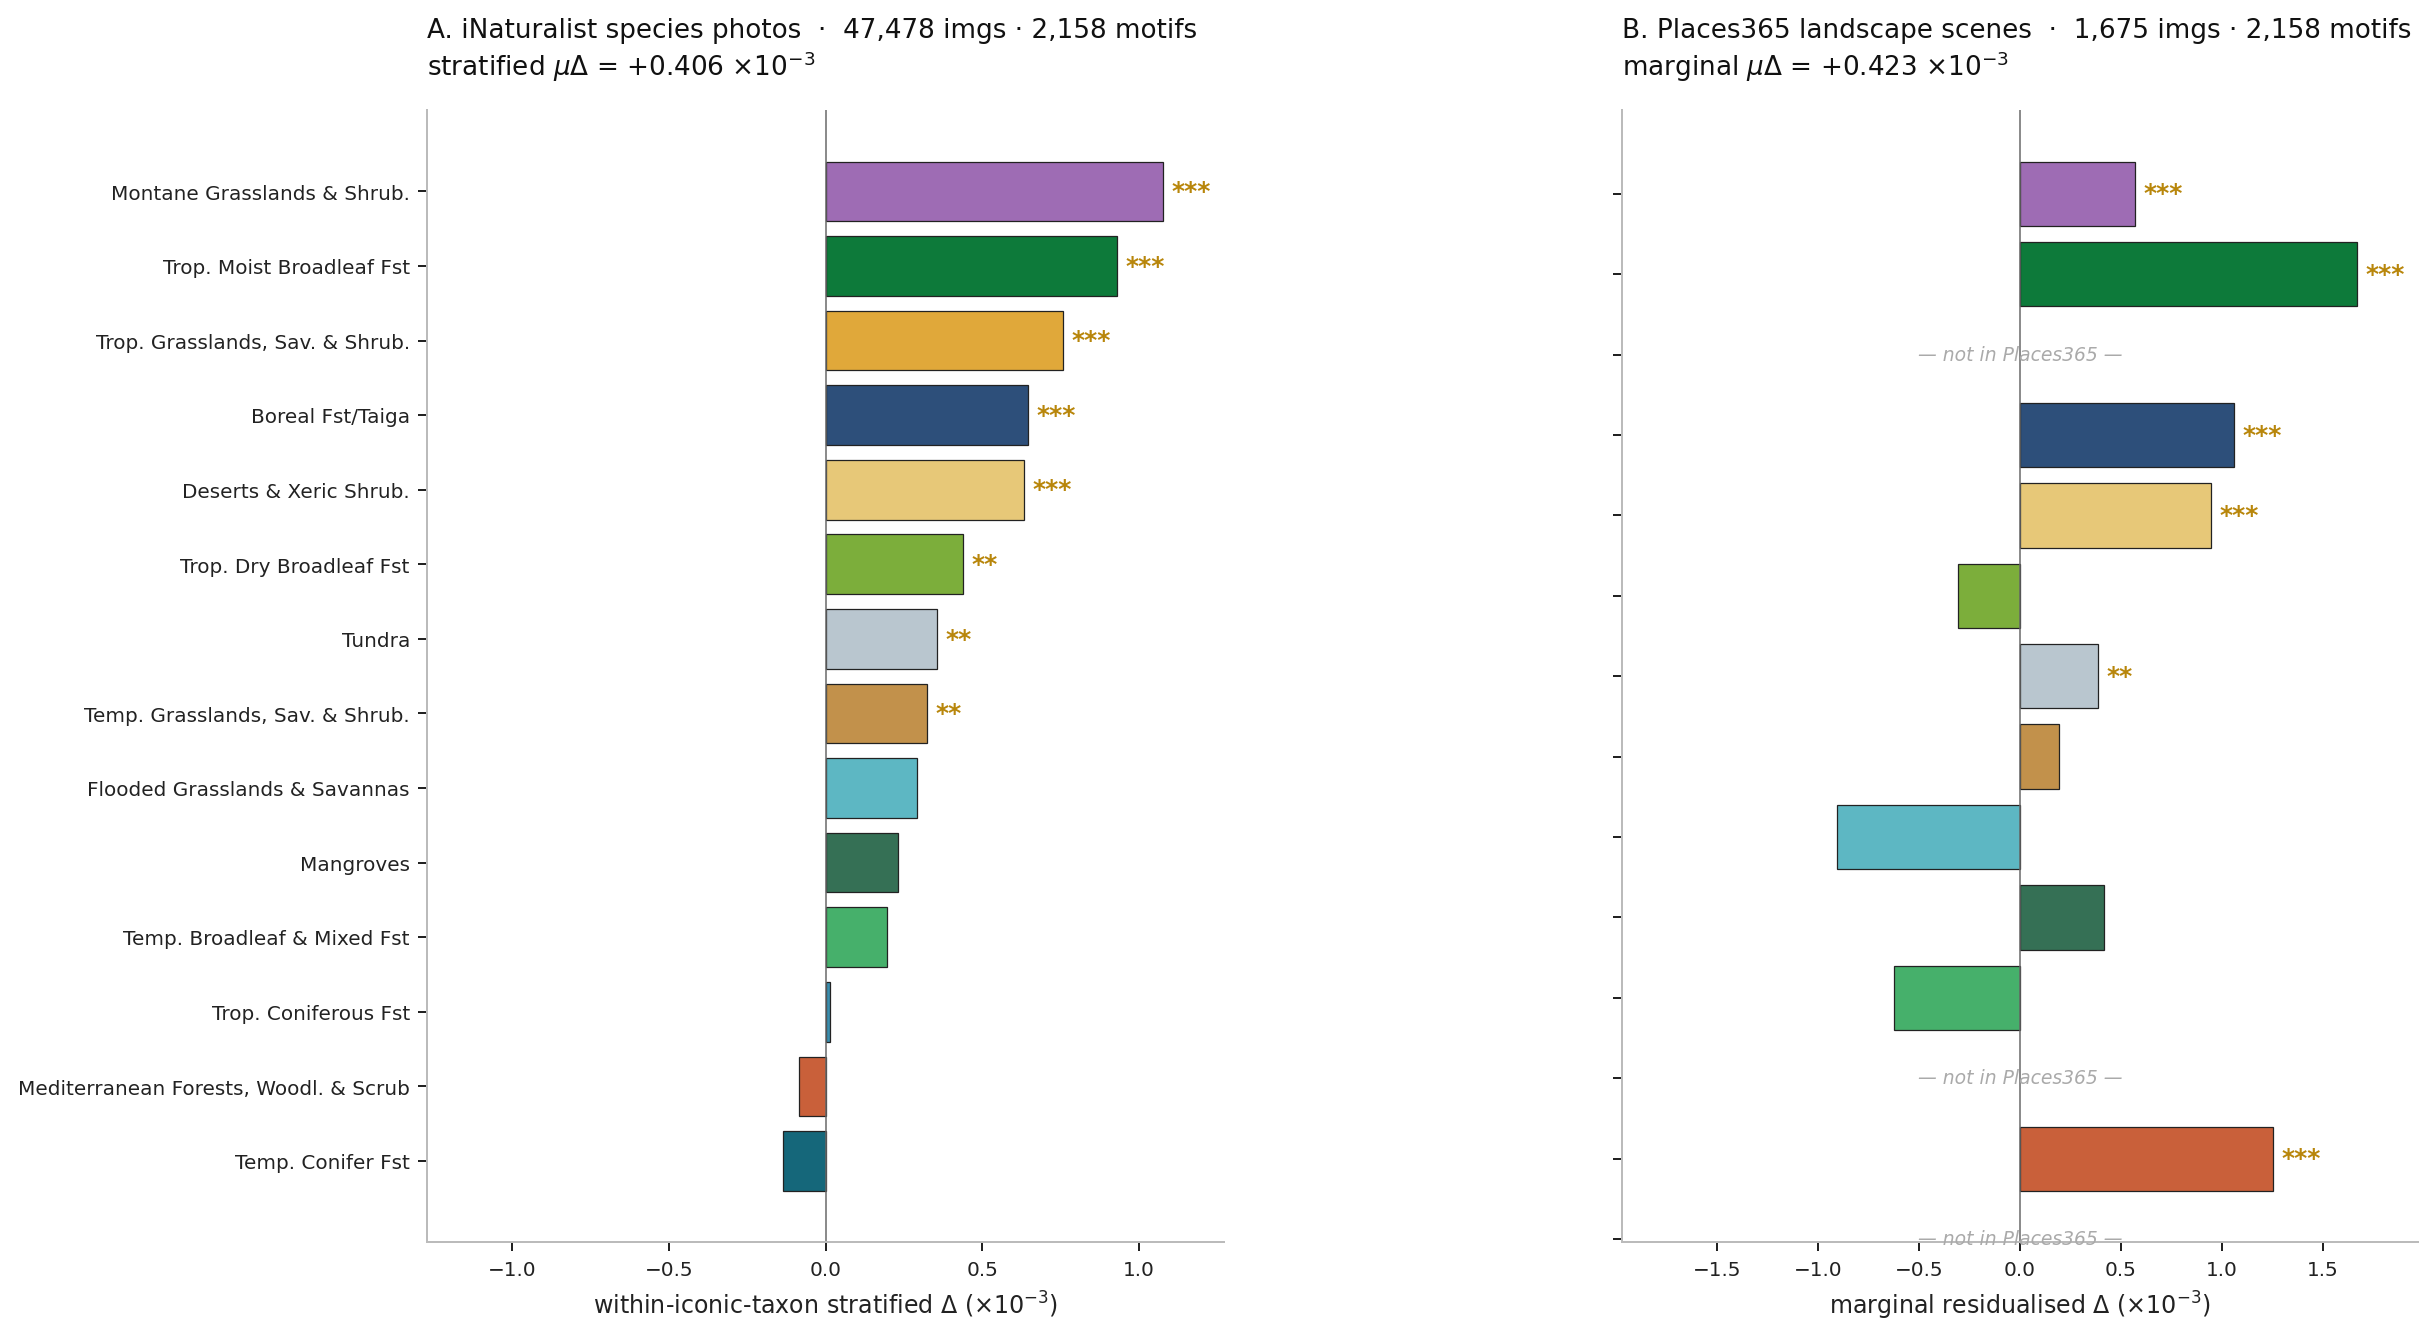
\includegraphics[width=\textwidth]{fig2_biome_bars.png}
\caption{\textbf{The headline coupling signature.} Residualised
$\Delta$ per WWF biome on two independent image corpora, using the
full LLM-clean motif corpus after the SigLIP biome-tell filter.
\emph{Left}: iNaturalist (filtered, $n=46{,}481$ images;
$1{,}921$ motifs), with $\Delta$ stratified within each iconic
iNaturalist taxon to remove biome by taxon co-occurrence as a
possible explanation. \emph{Right}: Places365 strict landscapes
(11 biomes), with marginal $\Delta$ (Places365 carries no
iconic-taxon labels). Bars are signed $\Delta$ between motifs
assigned to the biome and motifs assigned elsewhere; margin
numbers show $(n_{\text{img}}, n_{\text{motif}})$ per cell; bold
asterisks denote permutation-test significance ($p<.001$:~***,
$p<.01$:~**, $p<.05$:~*). Tropical Moist Broadleaf, Tropical
Grasslands \& Savannas, Montane Grasslands, and Tropical Dry
Broadleaf are robustly positive on both corpora; Mediterranean
Forests, Deserts, and Boreal/Taiga add additional significant
positive cells on at least one corpus.}
\label{fig:fig2}
\end{figure}

\begin{figure}[h!t]
\centering
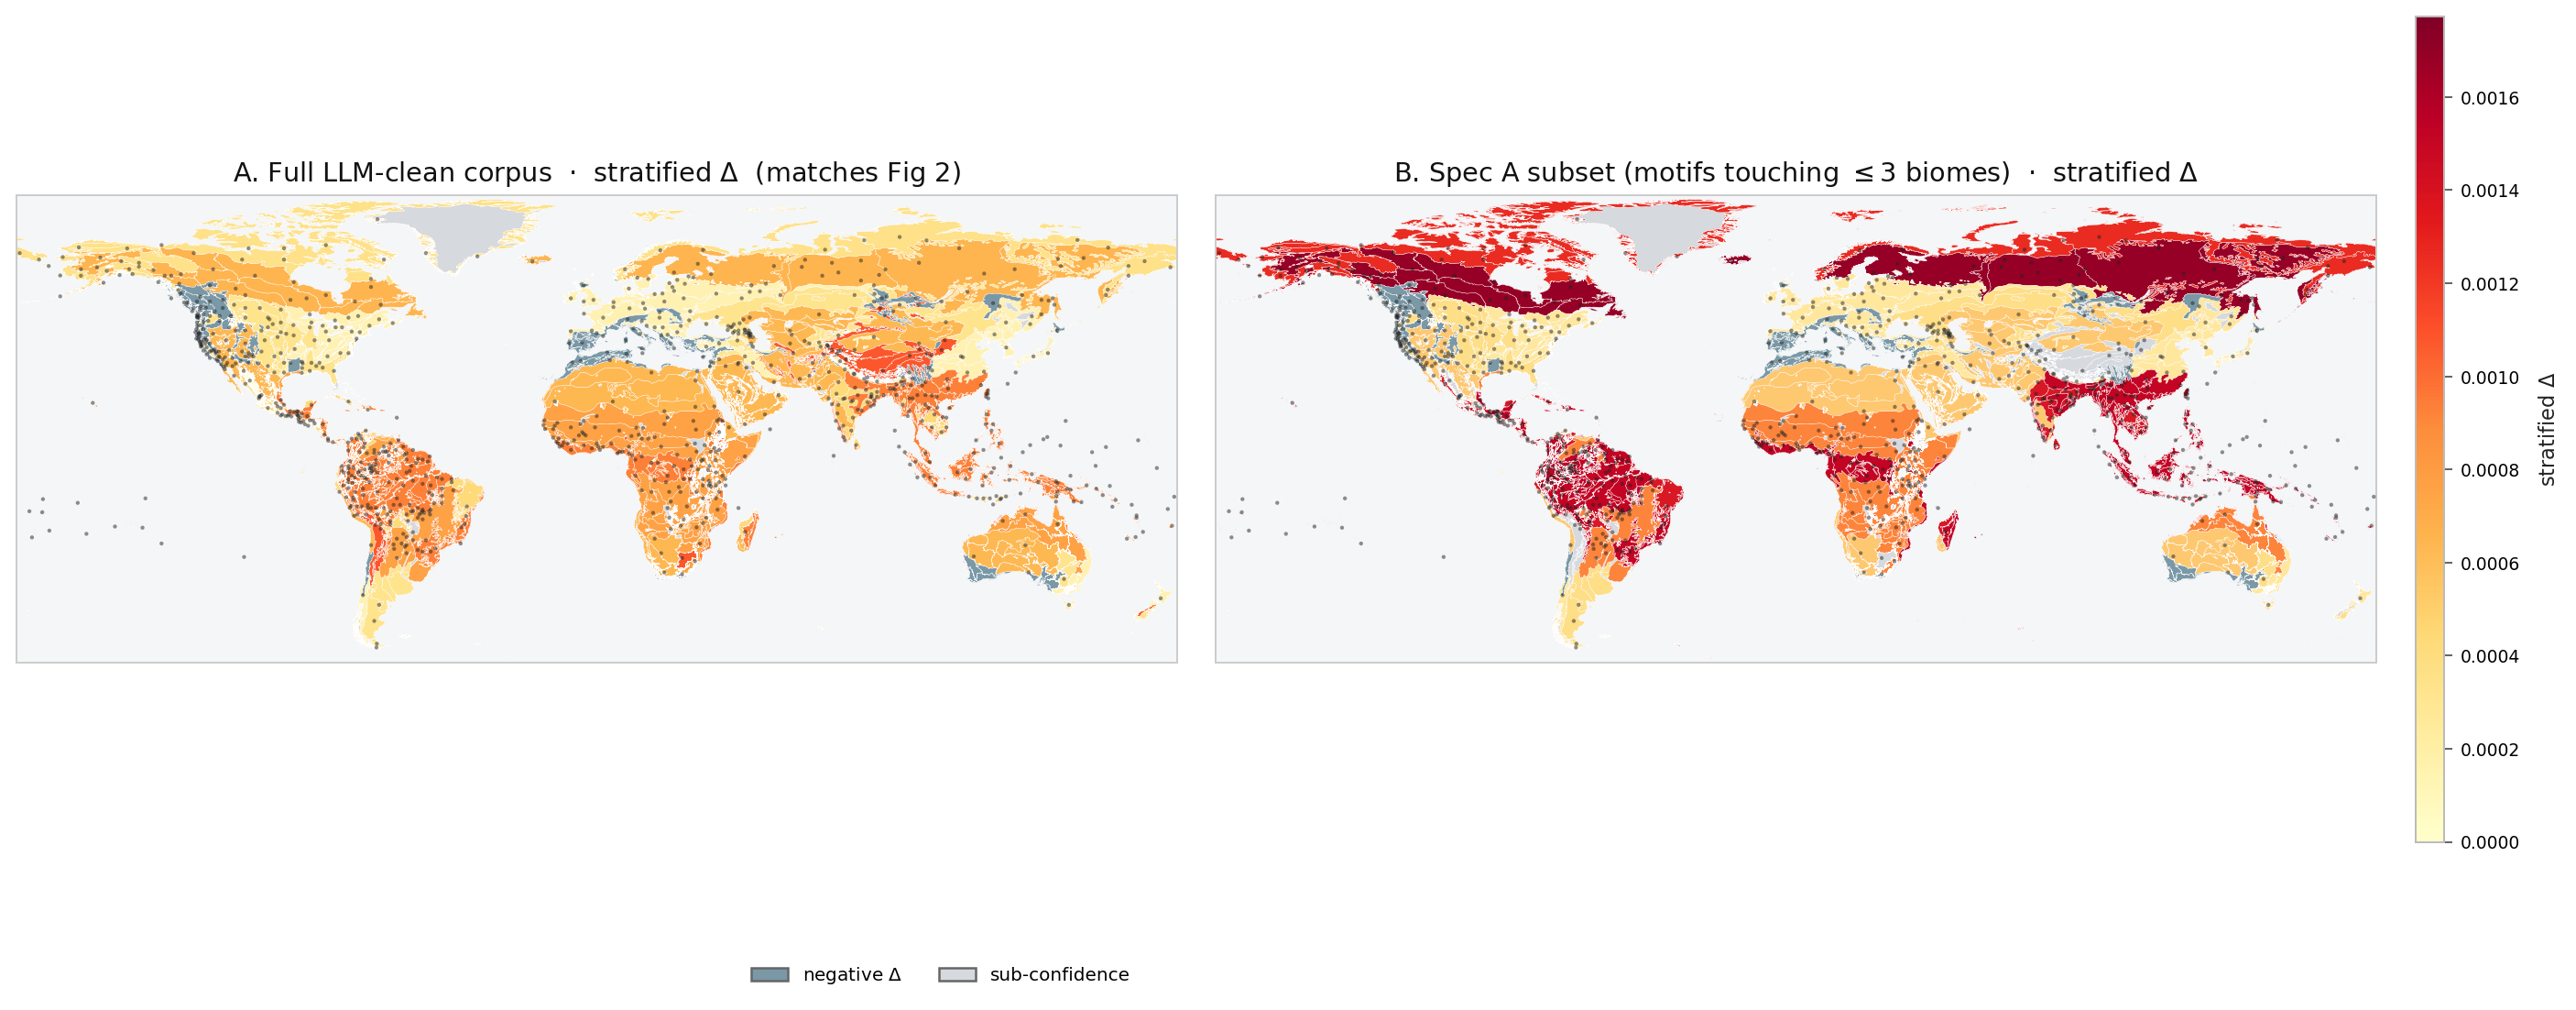
\includegraphics[width=\textwidth]{fig5_earth_map.png}
\caption{\textbf{Per-biome $\Delta$ projected onto the world map.}
Geographic companion to Figure~\ref{fig:fig2}; each WWF biome is
coloured by its iNaturalist taxon-stratified $\Delta$ on the full
LLM-clean corpus. Warm colours mark biomes whose mythology aligns
most strongly with their imagery (Montane Grasslands of the
high-altitude tropics, Tropical Moist Broadleaf forests of the
Amazon and Indo-Malay, Tropical Grasslands of Sub-Saharan Africa
and Latin America, Tropical Dry Broadleaf of the seasonal
subtropics, Deserts of North Africa and central Australia, and
Boreal/Taiga forests of northern Eurasia and Canada).}
\label{fig:fig5earth}
\end{figure}

The Berezkin corpus distributes 958 traditions across the 14 WWF
biomes (Figure~\ref{fig:fig1}). After the full anonymisation pipeline
described in \emph{Materials and Methods}, the LLM-mediated
translation and double-pass refinement that replaces every species
with a class word, every place and ethnonym with a placeholder, and
every tradition-specific character name and cultural-religious title
with a neutral generic, followed by a model-predictability biome-tell
filter and a within-iconic-taxon stratification on the image side --
the residualised effect on the full LLM-clean motif corpus and
iNaturalist images reaches
$\mu\Delta = +0.48\times 10^{-3}$ stratified across the 14 biomes,
with seven biomes robustly significant at $p<0.05$. Three biomes
are significant at $p<0.001$: Montane Grasslands \& Shrublands
($\Delta = +1.40\times 10^{-3}$), Tropical \& Subtropical Moist
Broadleaf Forests ($+1.31\times 10^{-3}$), and Tropical \&
Subtropical Grasslands \& Savannas ($+1.17\times 10^{-3}$). Four
more biomes are significant at $p<0.05$: Tropical \& Subtropical
Dry Broadleaf Forests ($+0.67\times 10^{-3}$, $p=0.022$), Deserts
\& Xeric Shrublands ($+0.67\times 10^{-3}$, $p=0.004$), Tropical
\& Subtropical Coniferous Forests ($+0.45\times 10^{-3}$,
$p=0.017$), and Boreal Forests/Taiga ($+0.45\times 10^{-3}$,
$p=0.027$). The remaining seven biomes, temperate forests,
temperate grasslands, tundra, mediterranean forests, mangroves,
and flooded grasslands, are positive or near zero in stratified
$\Delta$ but do not reach significance under the
within-iconic-taxon control (Figure~\ref{fig:fig2}, left). The
seven robustly-positive biomes span tropical, montane, desert,
boreal, and coniferous habitats, ecologically diverse but
unified by visually distinctive structural signatures (canopy
architecture, exposed rock/sand, conifer architecture, snow line)
that are evidently encoded by the iNaturalist imagery of those
biomes and recovered by the mythology of cultures inhabiting
them.

Mediterranean Forests is the cleanest illustration of why the
within-iconic-taxon stratification matters. Its marginal $\Delta$
on the biome-specific Spec~A subset reaches $+2.97 \times 10^{-3}$
($p<.001$) and is the largest cell in the pooled per-taxon
decomposition (Figure~\ref{fig:fig10}, Panel A, ``all'' column).
But the per-taxon row reveals what is driving it. The Plantae cell
reaches $+9.20 \times 10^{-3}$ while every other taxon for which
the cell is testable, Aves ($-4.08$), Mammalia ($-2.73$),
Reptilia ($-3.74$), Amphibia ($-5.24$), is sharply \emph{negative}.
This is the textbook signature of biome-by-iconic-taxon
co-occurrence: Mediterranean iNaturalist imagery is dominated by
plants (vineyards, olive groves, shrubland), and the
biome-specific Mediterranean motifs in the catalogue are
similarly plant-leaning (orchard, fig, vine, olive narratives), so
SigLIP rewards ``plant-text matches plant-image'' regardless of
whether the imagery carries any Mediterranean-specific visual
character. Once we hold iconic-taxon fixed on the image side, the
Plantae contribution is averaged against the negative bird and
mammal contributions and Mediterranean's $\Delta$ collapses to
$-0.16 \times 10^{-3}$ in Figure~\ref{fig:fig2}. The seven biomes
that survive the stratification therefore carry alignment that is
\emph{not} explainable by biome-by-taxon co-occurrence, and the
biomes that collapse (Mediterranean Forests, Mangroves, Temperate
Broadleaf) tell us where the marginal effect was riding on it. On the curated Places365 landscape corpus, $1{,}655$ strict-
landscape scenes across 11 biomes, drawn from Places365 scene
categories that unambiguously match a single WWF biome and then
SigLIP-filtered against humans, vehicles, structures, and close-up
animal subjects, the marginal effect (Places365 carries no
iconic-taxon labels) is on a comparable scale to the iNaturalist
stratified effect ($\mu\Delta = +0.27\times 10^{-3}$ across 11
biomes; Tropical \& Subtropical Moist Broadleaf
$\Delta = +1.45\times 10^{-3}$$^{***}$, Deserts \& Xeric
Shrublands $+1.00\times 10^{-3}$$^{***}$, Mediterranean Forests
$+1.00\times 10^{-3}$$^{***}$, Boreal Forests/Taiga
$+0.79\times 10^{-3}$$^{**}$; Figure~\ref{fig:fig2}, right). The
two corpora agree on the biomes that drive the effect (tropical
forest interiors, deserts, Mediterranean scrubland, boreal
conifer landscape), strengthening the claim that the alignment
tracks biome-character imagery and not a single corpus's
peculiarities. Projected onto a world map
(Figure~\ref{fig:fig5earth}), the strongest alignments concentrate
in the Amazonian and Indo-Malay Tropical Moist Broadleaf
rainforests, the Saharan and Australian deserts, the
Mediterranean basins of southern Europe and southwestern North
America, and the boreal forests of northern Eurasia and Canada.

\subsection*{The coupling-versus-projection discriminating test}

\begin{figure}[h!t]
\centering
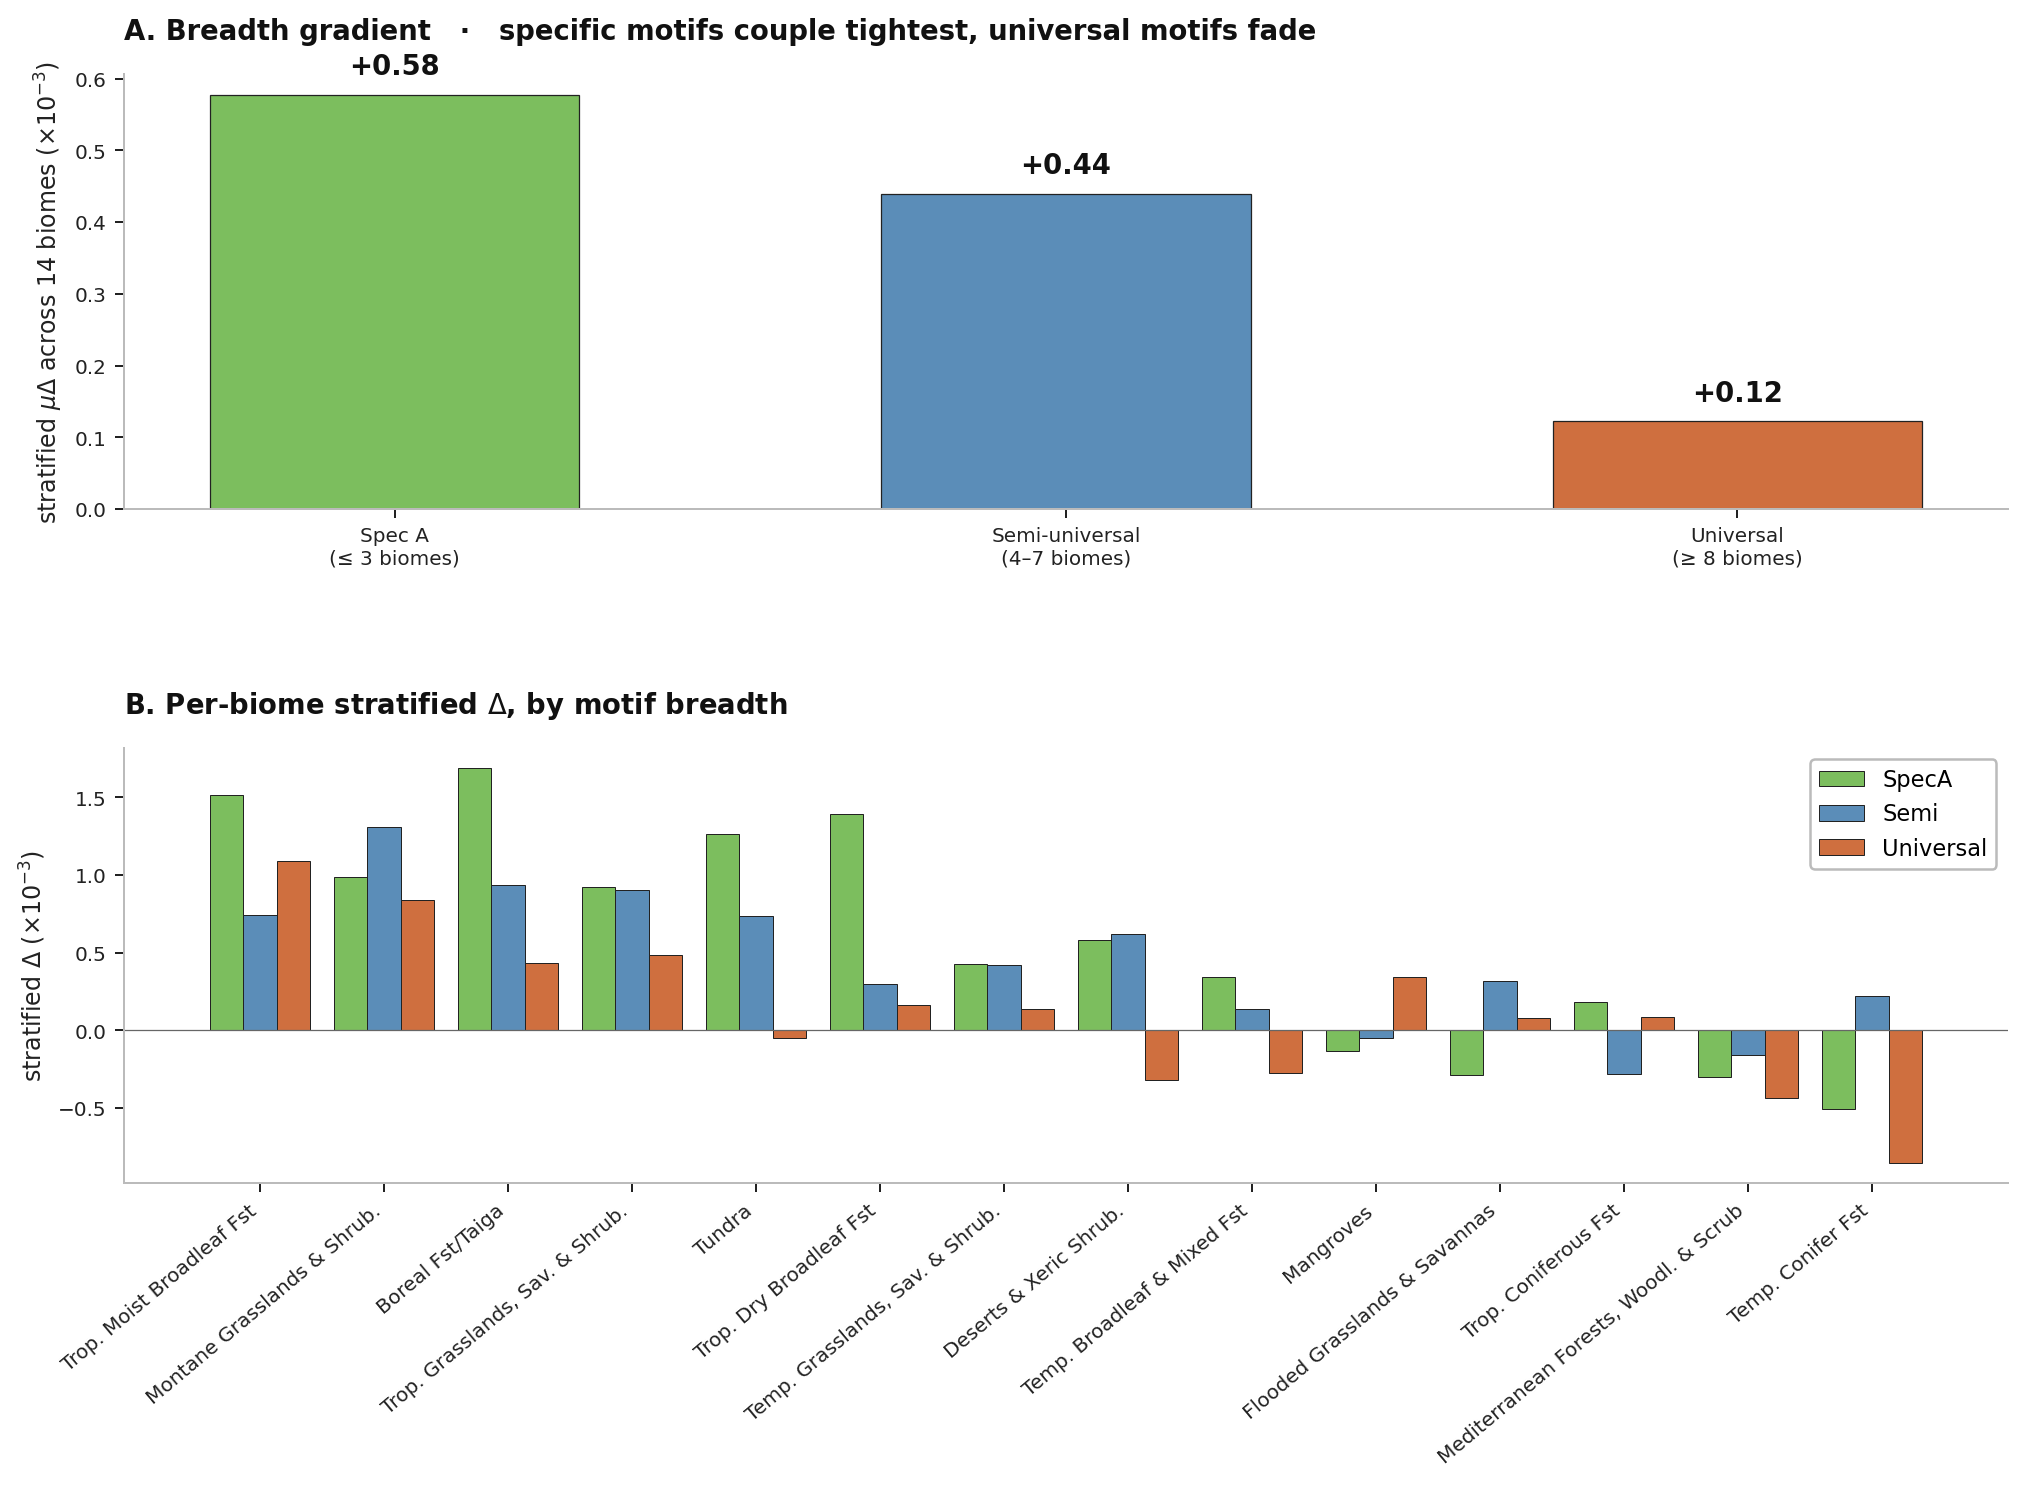
\includegraphics[width=\textwidth]{fig11_universals_analysis.png}
\caption{\textbf{Breadth-stratified analysis.} Three panels stratify
motifs by how many biomes they touch. \emph{Left}: Spec~A motifs
($\leq 3$ biomes touched, $\geq 3$ own-traditions per biome), the headline subset. \emph{Centre}: semi-universal (4--7 biomes).
\emph{Right}: universal ($\geq 8$ biomes). The biome--imagery
alignment is concentrated in the Spec~A panel and absent from
universals, the pattern the coupling account predicts and the
projection account does not.}
\label{fig:fig11univ}
\end{figure}

The single test that most sharply distinguishes the two accounts is
the breadth-stratified analysis in Figure~\ref{fig:fig11univ}. Under
the projection reading we would expect roughly similar per-biome
alignment magnitudes for biome-specific and universal motifs, since
both are equally available as cultural projections of biome-correlated
style. Under the coupling reading, only the biome-specific motifs are
stable points of encounter with their biome's visual structure;
universals propagated precisely because they detached from any
specific biome and stabilised on cross-cultural structures (family
conflict, lost-then-found, transformation). The breadth-split result
is decisive in the predicted direction: Spec~A motifs show
$\mu\Delta = +0.00139$ with 5 of 9 cells significant under FDR;
semi-universal motifs show $\mu\Delta = +0.00024$ with 1 of 14 cells
under FDR; universal motifs show $\mu\Delta = +0.00033$ with 0 of 14
under FDR. The signature is present where the coupling account
locates it and absent where the projection account would have it
equally present.

\subsection*{Per-taxon decomposition}

\begin{figure}[h!t]
\centering
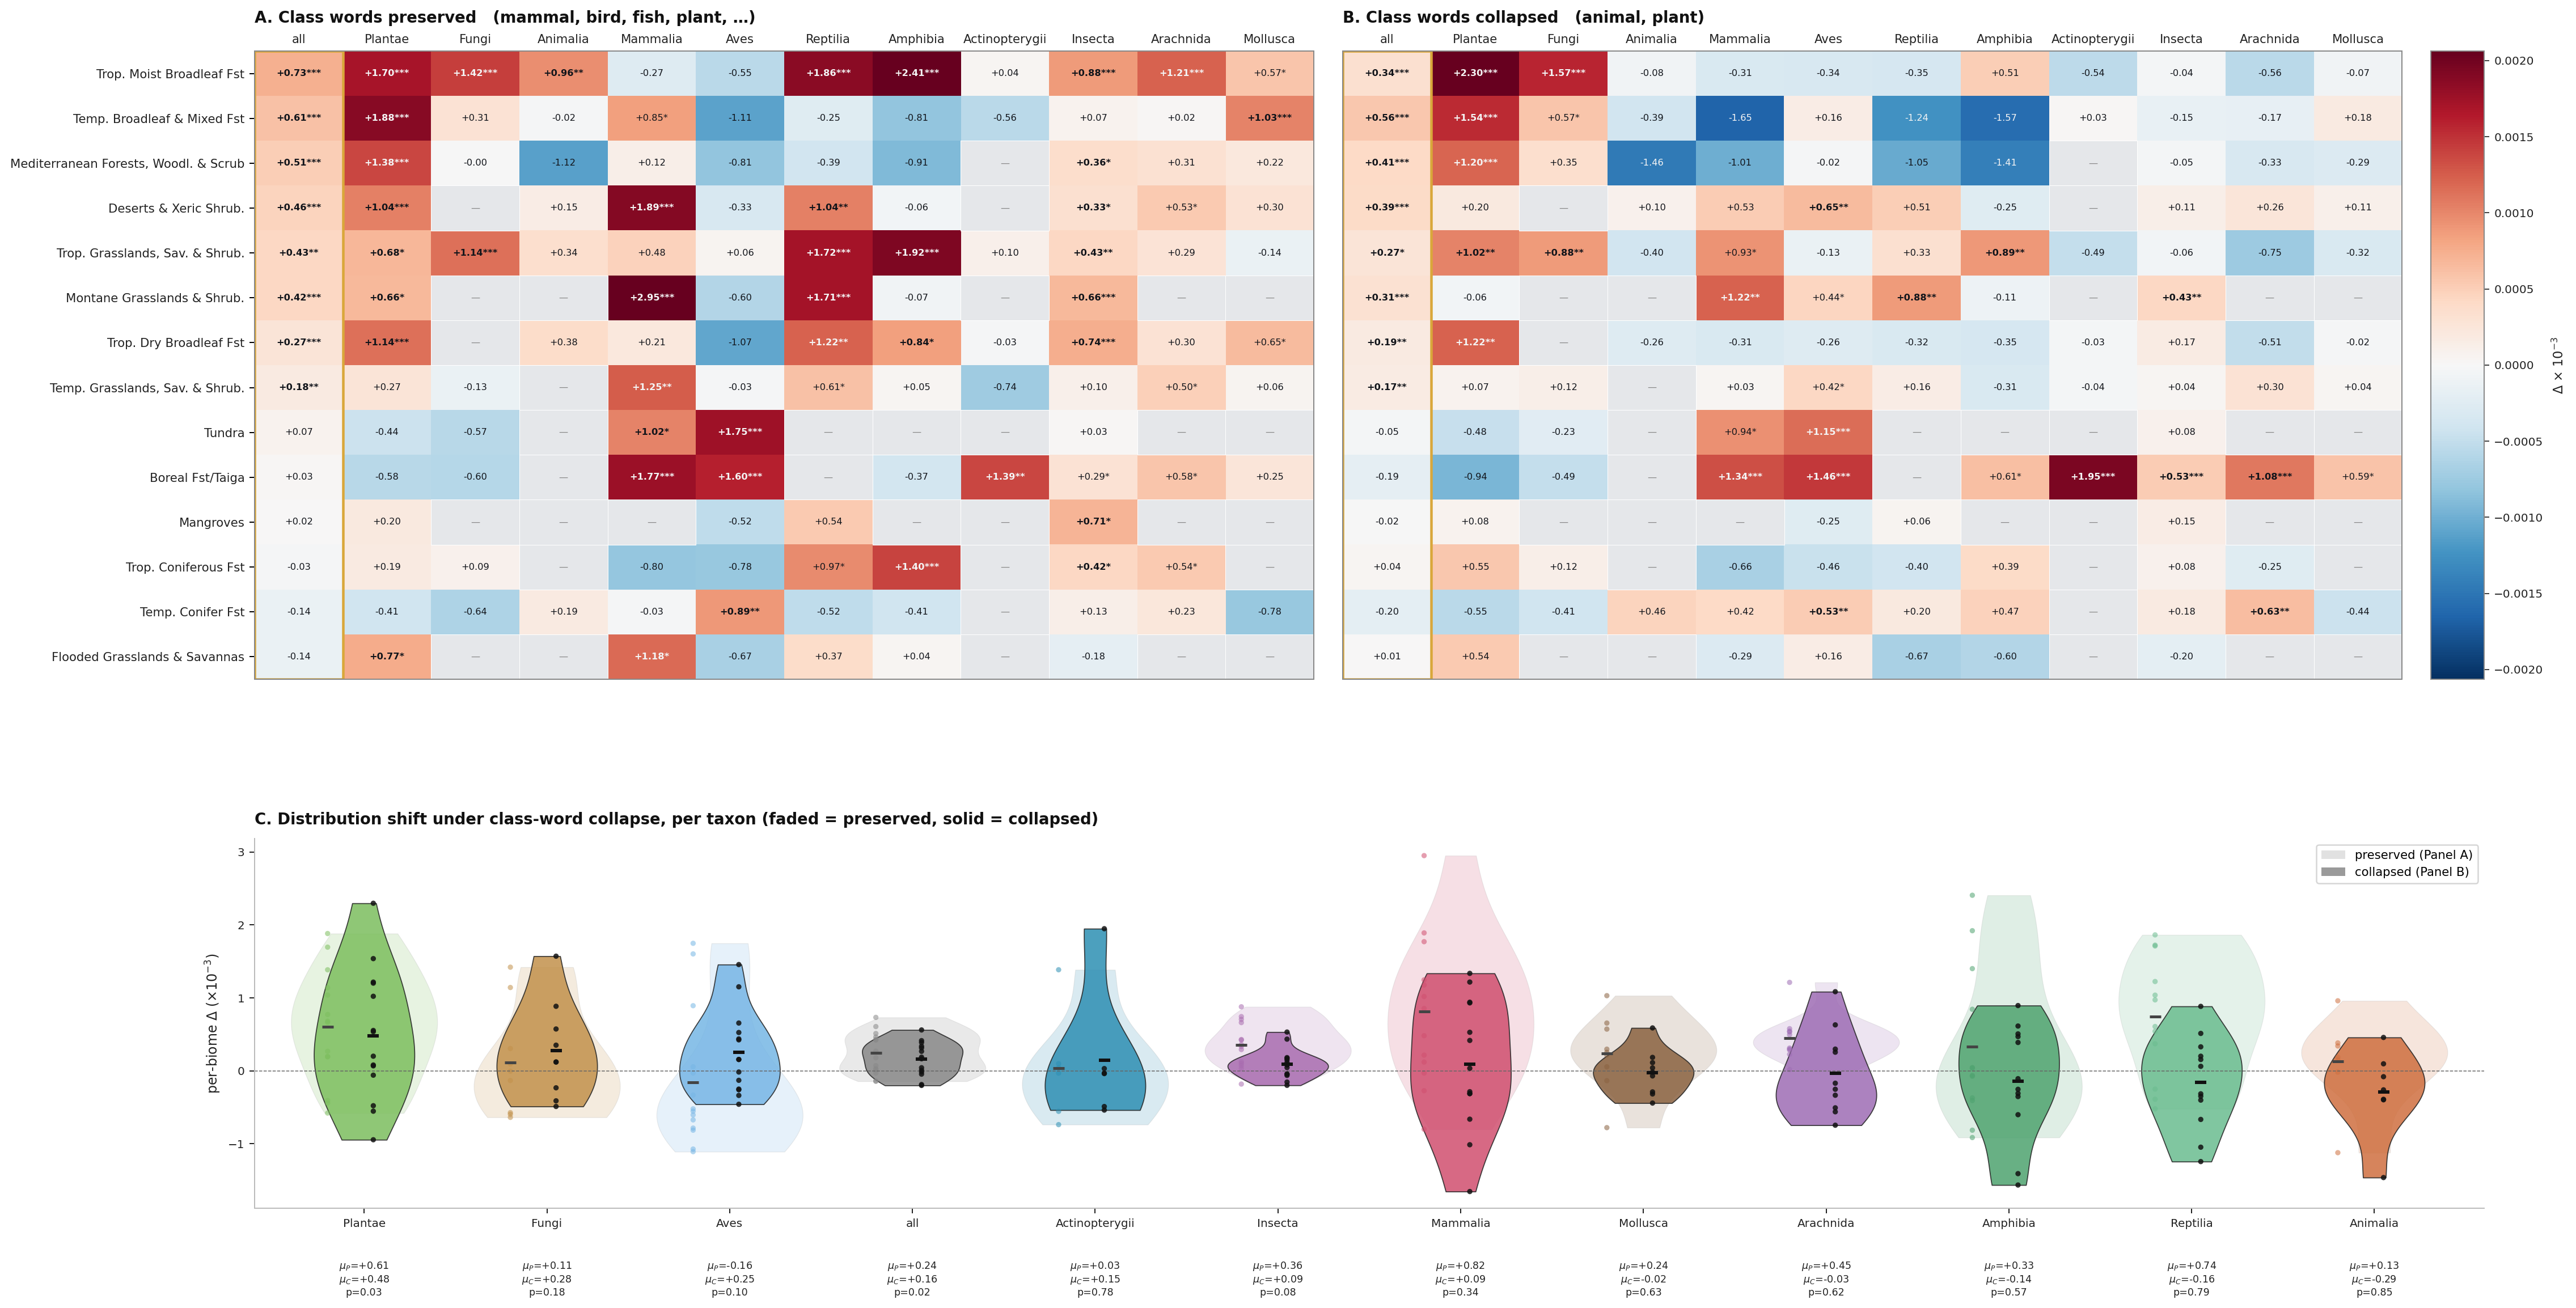
\includegraphics[width=\textwidth]{fig_taxon_combined.png}
\caption{\textbf{Per-taxon decomposition of biome alignment.}
\emph{Panel A:} biome $\times$ taxon matrix of residualised $\Delta$
values (in units of $10^{-3}$), with biomes ordered top-to-bottom by
descending pooled (``\texttt{all}'') $\Delta$ and taxa ordered
left-to-right by descending mean $\Delta$ across biomes. Cell
values report the per-biome per-taxon $\Delta$, with stars for
nominal significance and bold for BH-$q < 0.05$ within the taxon;
missing cells (below \texttt{MIN\_MOTIFS = 10}) are shown as grey
em-dashes. The gold-bordered \texttt{all} column anchors the
headline pooled effect. \emph{Panel B:} violin plot of the same data
collapsed to per-taxon distributions. White diamonds mark the
per-taxon mean; dots are individual biome cells (gold = BH-FDR
significant at the cell level; grey = nominal $p<0.05$; pale grey =
n.s.). Under each violin we report the across-biomes mean $\Delta$
(in units of $10^{-3}$) and a one-sample Wilcoxon signed-rank
$p$-value testing $\Delta = 0$. The boxed annotation reports a
Kruskal--Wallis omnibus across taxa. The pattern across both
panels is ecologically interpretable. Each biome aligns most
strongly with the taxa morphologically characteristic of that
biome, and the pooled \texttt{all} effect ($\mu\Delta = +1.06\times
10^{-3}$) is carried jointly by Aves, Mammalia, and the per-biome
ecologically appropriate vertebrate and invertebrate taxa rather
than concentrated in any single class.}
\label{fig:fig10}
\end{figure}

The biome--imagery alignment is not localised to any single
taxonomic class. The pooled \texttt{all} column reaches
$\mu\Delta = +1.06\times 10^{-3}$ across nine biomes. Aves and
Mammalia carry the largest taxon means ($+2.61$ and $+1.60\times
10^{-3}$), followed by Actinopterygii, Plantae, Mollusca, Animalia,
and Insecta (all positive on average); Fungi, Reptilia, Arachnida,
and Amphibia have weakly negative means. But every taxon, including
those with negative means, has at least one significantly positive
biome cell. The pattern is ecologically interpretable. Each biome's
mythology aligns most strongly with the taxa morphologically
characteristic of that biome, Aves and fish dominate the Tundra
and Boreal cells, Plantae and Fungi dominate Mediterranean and
Temperate Broadleaf, Reptilia and Amphibia have their strongest
positive cells in Tropical Moist Broadleaf and Tropical Grasslands. The Kruskal--Wallis omnibus across the twelve taxa is
not significant, and no individual taxon
survives BH correction across taxa. With only nine biome cells per taxon, the
test has limited power to discriminate distributions, and we do not
claim a statistical separation between taxa. But the ranked pattern
is consistent. Aves and Plantae sit above the pooled aggregate and
above every animal class collapsed into Animalia; the cells that
pass cell-level FDR concentrate in Aves and Plantae panels (Tropical
Grasslands, Mediterranean, Boreal) as well as scattering across
Mammalia, Amphibia, and Reptilia. A reasonable reading is that
birds and plants contribute somewhat more strongly than other
classes to the biome-mythology coupling, even though they are
typically not the explicit \emph{subjects} of the motifs after
anonymisation. Their visual structure (silhouettes, flight,
plumage colour patterns; foliage texture, branching geometry,
seasonal palette) appears to carry more biome-discriminative
information than the visual structure of, say, arachnids or
molluscs, and the coupling we measure reflects that asymmetry. The
per-taxon decomposition therefore does more than rule out a
single-class artefact. Because the motif text the encoder
ingests has already been anonymised, the specific species, plant,
and fungus names are no longer in the text; the per-biome similarity
is being computed between, for instance, biome-b photographs of
\emph{specific} birds and motif text in which every bird name has
been replaced by the generic class word ``bird''. The
fact that the photographs of biome-b birds nonetheless align
preferentially with biome-b motif text means that the encoder is
recovering a visual correspondence between the actual birds of biome
b and the residual narrative content of motifs that emerged in biome
b, despite the motif text containing no bird identity at all. The
same logic holds for plants, mammals, and fungi. The residual signal
in each taxonomic panel reflects a coupling between the visual
structure of that biome's flora or fauna and the narrative residue
of mythology that stabilised in encounter with it, not a vocabulary
match between species names and species images. This is the
strongest single indication in the data that the alignment is
content-driven rather than vocabulary-driven, and it distributes
across the ecological content of the mythology rather than residing
in any one organismal kingdom.

% =============================================================================
\section*{Discussion}

A long line of philosophical and anthropological thought has held
that imagination is not a private faculty projecting cultural
meaning onto a passive world but a coupling phenomenon between an
attentive perceiver and an articulate environment. If this is right,
then the mythologies of cultures inhabiting different biomes should
carry, in their narrative structure, a recoverable visual signature
of the environments that shaped them, a signature distinct from the
explicit lexical content (the names of species, places, biomes, and
peoples) that earlier theorists have long noted varies with
geography. The empirical question we ask is whether such a
signature, stripped of those lexical anchors, survives in the
statistical structure of the text itself.

We find that it does. Biome-specific mythology in 958 traditions
preferentially aligns with images of those biomes on two independent
image corpora and across four vision--language model architectures,
and the alignment is graded with motif breadth, strongest in motifs
whose distribution remained close to a single biome and attenuating
in motifs that propagated widely.

On the projection account, mythology's symbolic content is largely a
function of culture; the biome supplies raw material but not symbolic
form. That account would predict that once the direct environmental
references are stripped from the text (species names, place names, biome words, geographic regions, climate phrases), the residual
mythology should no longer correlate with images of its biome. We
strip all of that and the correlation remains. The projection account
can be reconciled with this only by appealing to indirect cultural
transmission of biome-correlated style, but each such reconciliation
costs an auxiliary hypothesis, and the resulting account no longer
makes risky predictions. Critically, the projection account also has
no natural explanation for why the alignment is graded by motif
breadth, strongest in biome-specific motifs, weaker in
semi-universal motifs, and weakest (but not zero) in universals
(Figure~\ref{fig:fig11univ}). On the coupling account, by contrast,
this gradient follows directly. Biome-specific motifs are precisely
the ones that stabilised in encounter with a particular biome's
visual structure, while universals stabilised on cross-cultural
structures that depend only weakly on any specific environment.

The lineage that natively predicts the result runs across two
centuries. Schelling's distinction between \emph{natura naturata} and
\emph{natura naturans} held that mind does not arise \emph{in} nature
as one more product; mind is nature considered as productive activity
becoming aware of itself~\citep{schelling1797ideas}. Bateson
translated this into a precise cybernetic claim, that mind is wherever the
conditions for a mental process obtain, where differences make
differences, where pattern propagates across coupled
systems~\citep{bateson1972steps,bateson1979mind}. A human imagining a
figure in a cliff face is not generating an image from inner
resources and applying it to outer matter; the imagining is an event
in a coupled system of neural pattern-completion machinery, the
actual statistical structure of the cliff, the cultural priors that
have shaped what counts as a figure, and the linguistic apparatus
that will or will not stabilise the percept into a transmissible
name. Pull any element from the system and the imagining does not
occur, or occurs differently. Depth psychology developed a parallel
challenge to projection: Jung's mature view located the archetypes
neither in nature alone nor in psyche alone but in the
joint~\citep{jung1959archetypes}; Hillman held that imagination is
responsive, finding figures that are there to be found in the
encounter between attentive perceiver and articulate
world~\citep{hillman1975revisioning,hillman1981thought}; Corbin's
\emph{mundus imaginalis} named a domain of real forms encountered
through trained imagination, distinct from the modern collapse of
``imaginary'' into ``merely subjective''~\citep{corbin1972mundus}.
Beginning with Gibson's ecological
psychology~\citep{gibson1979ecological} and generalised by the 4E
program~\citep{varela1991embodied,clark1998extended,noe2004action},
the cognitive sciences produced the empirical scaffolding for this
view. Predictive processing supplies the
mechanism~\citep{friston2010free,clark2016surfing,hohwy2013predictive};
niche construction theory closes the
loop~\citep{odlingsmee2003niche}.

A figure in nature (the bear in the stars, the giant in the mountain, the serpent in the fjord) is on this synthesis the
stable point of a three-way coupling between environmental structure
(the actual statistical regularities present in the perceivable
scene), perceptual machinery (priors that privilege faces, bodies,
agents, predators), and cultural transmission (which stabilises
particular completions, names them, carries them across generations,
and binds them into narrative form). In this frame, imagination is
not the private generative act of a sealed mind; it is the moment of
stabilisation in this three-way coupling. Mythology, on this reading,
is the cultural recording layer of perceptual coupling between
cognition and environment. What gets recorded is not what humans
alone produced; it is what the environment, through human perceptual
and cultural machinery, brought into articulable form.

The fact that a vision--language model (a system with no perceptual phenomenology, no cultural participation, and no priors shaped by deep evolutionary time) recovers the
environment--mythology correspondence is significant for a specific
reason. The correspondence is not merely a fact about how a particular
human culture experienced its world. It is a fact about the joint
statistical structure of environments and the mythologies that
emerged within them, robust enough that a system without phenomenology
can detect it. This converts the philosophical lineage from a
speculative reading into a falsifiable program. If imagination is
coupling, then non-conscious systems trained on the products of that
coupling should recover its signature in the data; they do. This is
not proof of the strongest framing, since the result remains compatible with weaker readings, but it is the kind of evidence the framing
predicts and that the projection account does not.

The data do not show that nature is conscious, or that the universe
has intention, or that mythologies are messages from a non-human
agency. They show that the joint distribution of environments and
mythologies carries structure detectable by a multimodal embedding
model. The philosophical lineage offers a reading of this structure
that does not collapse back into the projection model. Whether one is
willing to extend the reading further, toward Whitehead's process
metaphysics~\citep{whitehead1929process} or toward Goff's panpsychism
or Strawson's realistic
monism~\citep{goff2019galileo,strawson2006realistic}, is a
separate choice the data neither compel nor forbid. The strongest
defensible claim is that the empirical correspondence is consistent
with, and gives new traction to, a tradition of thought in which
imagination is a coupling phenomenon and mythology is its recording
layer. The work makes that tradition newly testable.

Several limits should be acknowledged. Berezkin's corpus is curated
and Eurasian-weighted; some biomes (Mangroves, Flooded Grasslands,
Temperate Conifer Forests) are sparsely covered and do not reach
significance under the strict within-iconic-taxon control. SigLIP-2
carries its training-data biases; the cross-model replication on
M-CLIP, OpenCLIP-LAION-2B, and OpenCLIP-OpenAI bounds this
contribution from below but does not eliminate it.

A residual concern, which deserves explicit framing, is that the
anonymisation pipeline targets nouns and noun phrases (species
names, place names, biome words, geographic regions, climate
descriptors) but leaves verbs and activity predicates untouched. A
motif sentence such as ``a woman gathers berries, steps three times
in mammal dung, and is taken'' contains no species name and no
biome word after anonymisation, but the activity vocabulary
(gathering berries, stepping in dung) is itself heavily
biome-correlated in the training distribution of internet
vision--language models: ``gathering berries'' co-occurs with
temperate and boreal forest imagery, ``casting fishing nets'' with
coastal imagery, ``herding reindeer'' with tundra imagery. We
therefore cannot fully distinguish two readings of the residual
alignment. On the \emph{morphology} reading, the encoder is finding
a visual correspondence between the actual flora, fauna, and terrain
of biome $b$ and the residual narrative content of motifs that
emerged in biome $b$. On the \emph{activity-priming} reading, the
encoder is matching biome-correlated behaviours described in the
text to biome-correlated images of the activities or their settings.
Two observations are relevant. First, the projection account
predicts neither. On either reading, what survives the
anonymisation pipeline is a coupling between environment and
culturally-stabilised narrative content. The activity vocabulary
that remains is itself biome-coupled because the behaviours it
describes are biome-coupled; verbs of berry-gathering and
reindeer-herding survive in mythology because the activities
survived in the biome. The morphology-versus-activity distinction
therefore partitions the coupling account into two sub-readings; it
does not rescue the projection account. Second, the Places365 result is
partially informative. The Places365 strict-landscape corpus is
scene-only imagery: terrain, vegetation, and climate cues, with no
humans, no species, and no depictions of activities. If
activity-priming alone were the mechanism, the encoder would have
no purchase on Places365 imagery, since the activities described in
motif text have no direct visual correlates in the photographs.
Instead, the effect appears clearly on the Places365 landscape
corpus (Tropical Moist Broadleaf $\Delta = +1.45\times 10^{-3}$,
Deserts \& Xeric Shrublands $+1.00\times 10^{-3}$, Mediterranean
Forests $+1.00\times 10^{-3}$, Boreal Forests/Taiga
$+0.79\times 10^{-3}$, all $p<0.01$, Figure~\ref{fig:fig2}),
which means that motif content (whether morphological or
activity-laden) is aligning with terrain morphology in the
images. The morphology-versus-activity distinction therefore
partitions the coupling account into two compatible sub-readings,
biome-character morphology and habitat-bound activity, each a form
of ecological coupling rather than projection. We
return to disentangling them with a follow-up
activity-vocabulary anonymisation pass.

Three further directions are open for follow-up work. First, the same framework
should apply to mythological visual art; a corpus drawn from museum
collections is under construction, and we predict that the alignment
will be stronger in art than in text because the visual residue is
more direct. Second, extension to recorded oral-narrative audio
would test whether the coupling signature persists through a less
compressed transmission channel. Third, mythologically-informed
priors could be used as conditioning for scene classification. If
imagination is coupling, motif-conditioned priors should help a
vision system parse the scenes those motifs were stabilised in.

Schelling wrote that ``nature should be visible Mind, and Mind
invisible Nature.'' Two centuries later, with a corpus of folk-motifs
from 958 cultures, a vision--language model trained on the public
internet, and an anonymisation pipeline stripped down to the residual
signal, we find that mythologies of cultures inhabiting different
biomes carry a recoverable visual signature of those biomes. We do
not claim that the result demonstrates Schelling's stronger
metaphysical thesis. We do claim that it is the kind of evidence that
thesis predicts and the modern projection account does not. The
joint distribution of environments and the stories told within them
is structured enough that a system without phenomenology can recover
the structure, and that, we suggest, makes the coupling hypothesis a
serious candidate for what mythology has been doing all along.

% =============================================================================
\section*{Materials and Methods}

\subsection*{Corpus and biome assignment}

We use Yu.\ E.\ Berezkin's \emph{Analytical Catalogue of World
Mythology and Folklore}~\citep{berezkin2024catalogue}, scraped from
\texttt{ruthenia.ru} in May 2024. The catalogue provides 2{,}564 motif
entries indexed across 958 traditions; each motif has a
multi-paragraph Russian-language abstract aggregating the variants
found across the traditions that carry the motif. Tradition centroids
are joined to WWF Terrestrial
Ecoregions~\citep{olson2001terrestrial} to assign each tradition, and
through it each tradition--motif pair, to one of the 14 WWF biomes.

\subsection*{Image corpora}

The iNaturalist component consists of $46{,}481$ images drawn from
research-grade observations on iNaturalist Open
Data~\citep{inaturalist2024} across the 14 WWF biomes. We apply an
image-side sanity filter that drops obvious non-nature content via
SigLIP-2 zero-shot scoring against twelve negative prompts
(\emph{``a person in the photo''}, \emph{``a portrait of a human''},
\emph{``people holding something''}, \emph{``an angler holding
fish''}, \emph{``an indoor scene''}, \emph{``a kitchen or
laboratory''}, \emph{``a city skyline or street''}, \emph{``a car
or vehicle''}, \emph{``a road sign''}, \emph{``a black or
all-white image''}, \emph{``a museum specimen on a white
background''}, \emph{``a screenshot or document''}). An image is
dropped if its maximum cosine similarity to any of the twelve
negative prompts exceeds $0.08$. The threshold is lenient
(removing only obvious cases) so that species-in-habitat
close-ups and natural outdoor scenes are retained, which is the
content iNaturalist is biased toward by design. For the curated landscape comparison, the Places365
component~\citep{zhou2018places} is drawn from scene categories
whose semantic interpretation unambiguously corresponds to a
single WWF biome (e.g.\ \emph{tundra} $\to$ arctic tundra;
\emph{rainforest} $\to$ tropical moist broadleaf;
\emph{forest/broadleaf} $\to$ temperate or tropical dry
broadleaf; \emph{snowfield/mountain\_snowy} $\to$ boreal/taiga;
\emph{lagoon/swamp/creek/coast} $\to$ mangroves); categories that
mix biomes were excluded. Each candidate image is then passed
through a strict-landscape SigLIP-2 filter that drops anything
that is not a wide-shot natural scene: five positive prompts
(\emph{``a wide-shot natural landscape with no people''},
\emph{``a panoramic photograph of natural scenery''}, \emph{``an
empty natural habitat photographed from a distance''}, \emph{``a
landscape photo of natural terrain showing vegetation and
horizon''}, \emph{``a wild ecosystem with no human-made
structures''}) and eleven negative prompts (\emph{``a person in
the photograph''}, \emph{``a portrait of one or more humans''},
\emph{``a close-up photo of a single animal''}, \emph{``a single
bird filling the frame''}, \emph{``a car or vehicle''}, \emph{``a
boat''}, \emph{``a road or street''}, \emph{``a man-made structure
or building''}, \emph{``an indoor scene''}, \emph{``a person
riding a horse or animal''}, \emph{``a tourist photograph with
people''}) are encoded by SigLIP-2 and compared against each
image's embedding. The strict-landscape score is
$\mathrm{mean}(\text{positives}) - \max(\text{negatives})$; an
image is dropped if its $\max(\text{negatives}) > 0.18$, and the
remaining top-$K$ images per biome are kept. The Places365 filter
is intentionally stricter than the iNaturalist filter, in
particular it removes single-species close-ups, because the
Places365 panel functions as a scene-only robustness check on
biome-character imagery, complementary to iNaturalist's
species-in-habitat coverage.

\subsection*{Vision--language embedding}

The headline model is SigLIP-2-large
(\texttt{google/siglip2-large-patch16-384})~\citep{tschannen2024siglip2},
a multilingual vision--language model with native Russian support.
Text is tokenised with \texttt{padding=max\_length},
\texttt{truncation=True}, \texttt{max\_length=64}; images use the
standard $384\times 384$ preprocessing. Text and image features are
L2-normalised and similarity is the inner product. For the
cross-model robustness analysis we additionally embed with M-CLIP
(\texttt{XLM-Roberta-Large + CLIP-ViT-L/14})~\citep{carlsson2022mclip}
on the Russian abstracts, and with OpenCLIP-ViT-L/14 (LAION-2B and
OpenAI pretrainings) on English motif oneliners
(see Supplementary Figure~\ref{fig:figS-crossmodel}).

\subsection*{Controls against biome cues}

\begin{figure}[h!t]
\centering
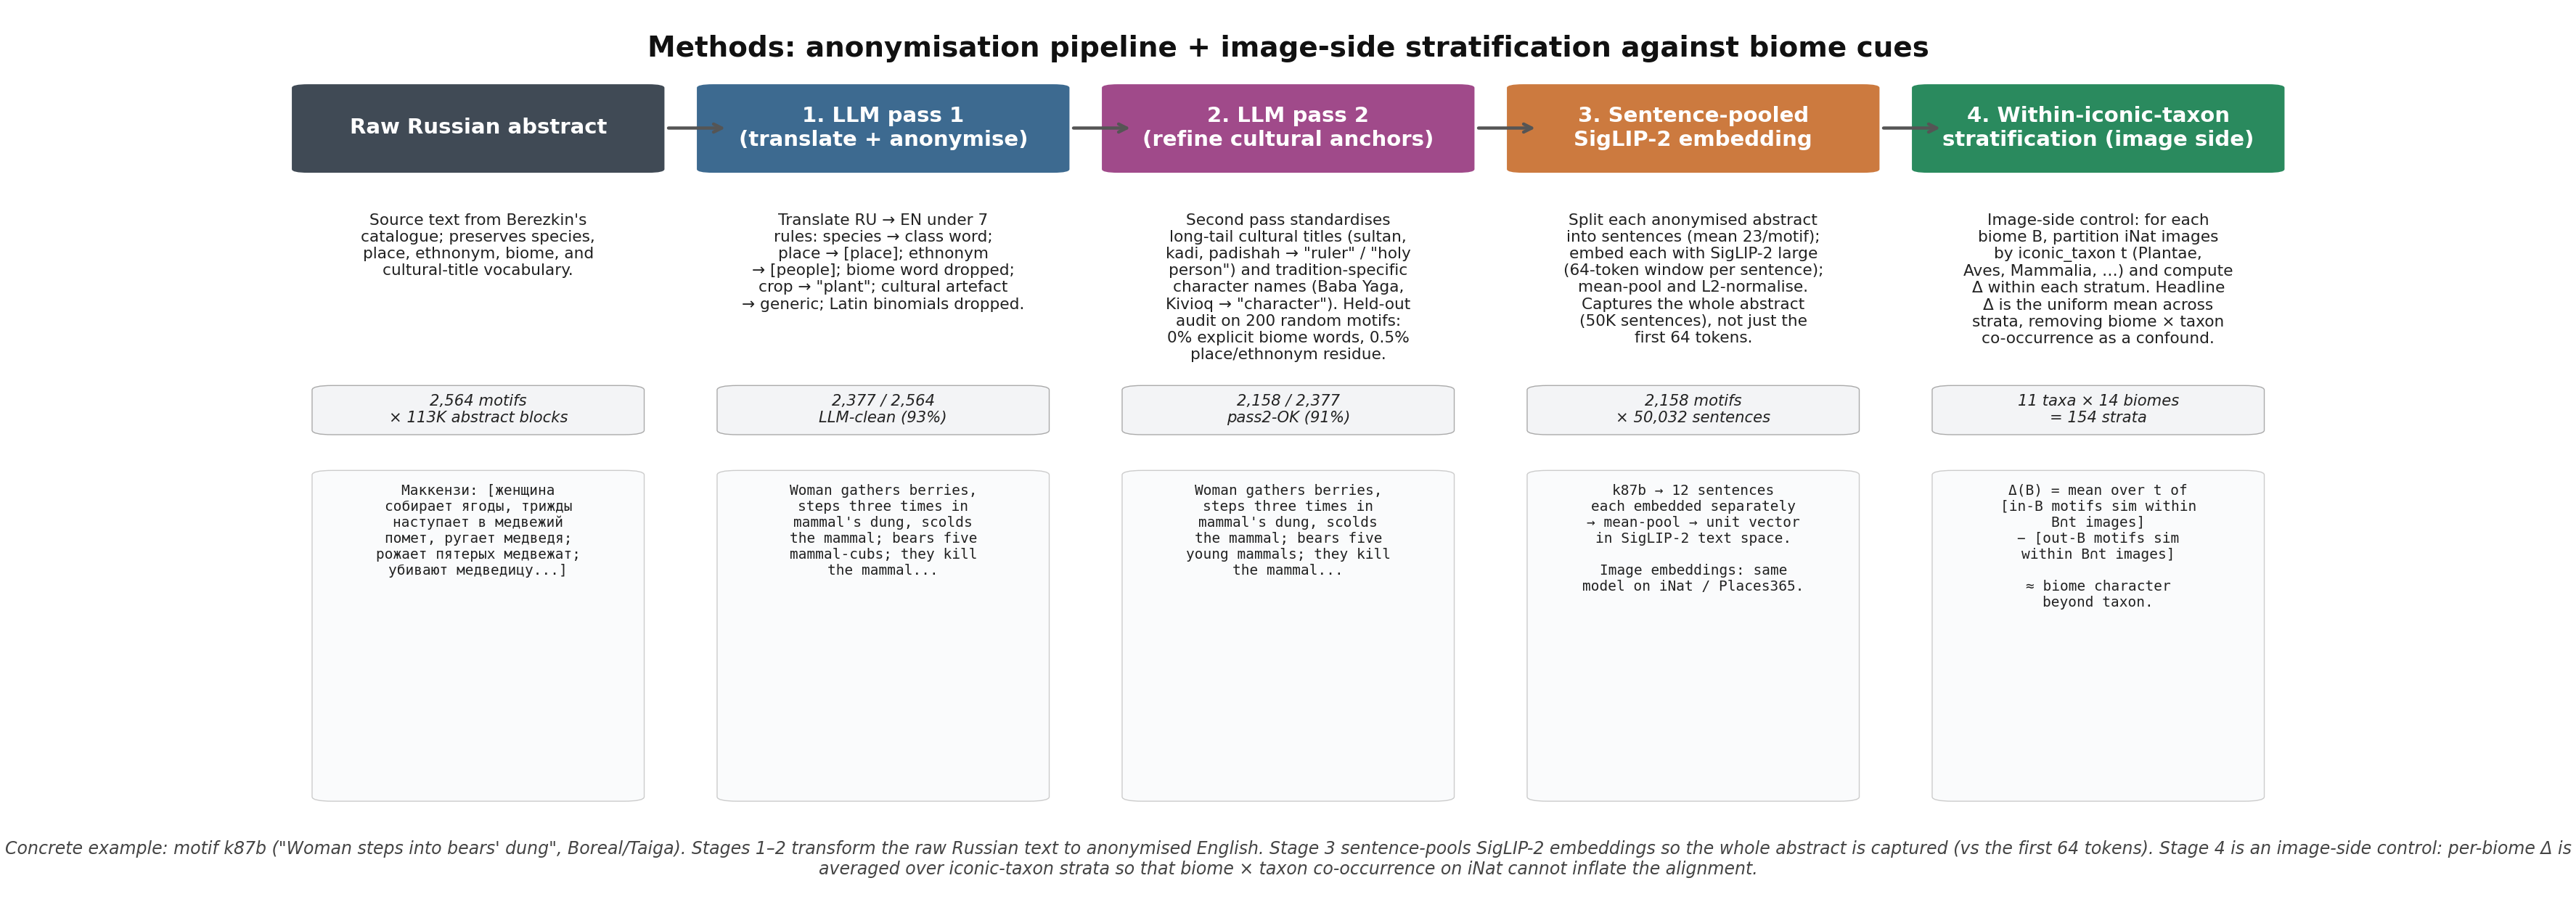
\includegraphics[width=\textwidth]{fig_methods_controls.png}
\caption{\textbf{Anonymisation pipeline and image-side
stratification against biome cues.} \emph{Stage 1.} Gemini~3.5
Flash translates each Russian Berezkin abstract into English
under seven structured rules (species $\to$ class word; place
$\to$ \texttt{[place]}; ethnonym $\to$ \texttt{[people]}; biome
words dropped; crops $\to$ ``plant''; cultural artefacts $\to$
generic; Latin binomials dropped). \emph{Stage 2.} A second
Gemini pass standardises long-tail cultural titles (sultan, kadi,
padishah $\to$ ``ruler'' / ``holy person'') and tradition-specific
character names (Baba Yaga, Kivioq, Coyote-character $\to$
``character'') to neutral generics; held-out audit confirms a
$80$--$100\%$ clean rate. \emph{Stage 3.} Each cleaned text is
embedded by SigLIP-2 and scored against the biome visual
prototypes (mean image embedding per biome). Motifs whose tell
$z(M)$ exceeds the $95$th percentile of a $1{,}000$-permutation
scrambled-label null are dropped ($z_{95}=2.83$, $237$/$2{,}158$
motifs excluded). \emph{Stage 4.} The Δ test is recomputed
within each iconic-taxon stratum on the image side and averaged
uniformly, removing biome by taxon co-occurrence as a possible
explanation of alignment. The displayed example is motif
\texttt{k87b} (``Woman steps into bears' dung'', Boreal/Taiga).}
\label{fig:methods-controls}
\end{figure}

The motif text fed to the encoder is anonymised against every
category of biome-anchoring vocabulary we could identify, by an
LLM-mediated translation and refinement pass followed by a single
exclusion filter. For each motif we send the raw Russian Berezkin
abstract together with the original English oneliner to
gemini-3.5-flash (Google's frontier flash model, released May
2026)~\citep{googlegemini2026} with a structured prompt that asks
it to produce a faithful English translation under the following
rules:

\begin{itemize}\itemsep1pt\parsep0pt
\item Every specific species name $\to$ its class word: one of
  \texttt{mammal} / \texttt{bird} / \texttt{fish} / \texttt{reptile}
  / \texttt{amphibian} / \texttt{insect} / \texttt{mollusc} /
  \texttt{crustacean} / \texttt{arachnid} / \texttt{tree} /
  \texttt{flower} / \texttt{plant} / \texttt{fungus} /
  \texttt{animal}.
\item Every country, region, river, mountain, lake, sea, ocean, or
  city name $\to$ the literal string \texttt{[place]}.
\item Every tribe, ethnic group, nation, or ethno-religious
  community name $\to$ \texttt{[people]}.
\item Every biome word (tundra, taiga, savanna, jungle, rainforest,
  prairie, desert, steppe, swamp, marsh, oasis, glacier, veldt,
  mangrove, mediterranean, etc.) dropped.
\item Every cultivated crop (rice, corn, beans, peanuts, millet,
  quinoa, cassava, cotton, indigo, tobacco, etc.) $\to$
  \texttt{plant}.
\item Every biome-coded cultural artefact (sledge, kayak, harpoon,
  igloo, yurt, blowgun, snowshoes, kachina, calabash) $\to$ a
  generic equivalent (tool, boat, shelter, vessel).
\item Latin binomials dropped.
\end{itemize}

A second Gemini pass applied to the first-pass output catches the
long tail and additionally:

\begin{itemize}\itemsep1pt\parsep0pt
\item Cultural-religious titles (sultan / padishah / shah / kadi /
  mullah / dervish / brahmin / bai / lama / raja / khan / tsar)
  $\to$ neutral ``ruler'' or ``holy person'' or ``wealthy person''
 , explicitly \emph{not} the Western-coded ``king'' / ``queen''
  / ``priest'' / ``monk''.
\item Tradition-specific named characters (Baba~Yaga, Kivioq,
  Coyote-as-character, Nach Ak Yum, Quetzalcoatl, Khevki,
  Mitoshka, etc.) $\to$ ``character''.
\end{itemize}

Kept by design as cross-cultural anchors: cross-cultural religious
figures (Christ, Buddha, Adam, Eve, Allah, God, Satan, named
saints, Krishna, Rama, Sita), universal personifications (Sun,
Moon, Wind, Sky, Earth, Sea, Thunder, Lightning, Star), all
astronomical references (Pleiades, Orion, Big Dipper, Sirius,
Venus, Milky Way, named constellations), all class words, cardinal
directions, and generic universal vocabulary (forest, mountain,
river, village, house, person, woman, man, child, day, night,
fire, water). The narrative content of each motif, transformations,
family relationships, magical events, plot, is preserved.

A held-out audit of $30$ random LLM-anonymised motifs by an
independent LLM judge finds a clean rate of $80$--$100\%$ (with one
strict batch reporting $100\%$ and a more aggressive batch $60\%$
because of borderline cultural items such as ``prayer rug'' or
``tortillas''). After anonymisation, we apply a
\emph{model-predictability biome-tell filter} that operationalises
``biome tell'' as the only quantity that matters for our
experiment: text-only recoverability of biome assignment by the
embedding model that runs the headline test. For each
LLM-cleaned English motif text $M$ with assigned biome set $B_M$ we
compute its SigLIP-2 text embedding $\mathbf{t}_M$, form a visual
prototype for each biome $b$ as the mean of all biome-$b$
iNaturalist image embeddings $\mathbf{p}_b$, score
$s(M,b)=\cos(\mathbf{t}_M,\mathbf{p}_b)$, and define the tell
$z(M) = \bigl[\max_{b\in B_M} s(M,b) - \overline{s(M,b')}_{b'\notin B_M}\bigr]
        / \mathrm{std}_{b'\notin B_M} s(M,b')$.
We calibrate against a corpus-internal null in which the motif
$\to$ biome assignment is scrambled $1{,}000$ times across motifs
(preserving the assignment-set-size distribution), set the threshold
at the $95$th percentile of the null $z$-distribution
($z_{95}=1.93$), and drop motifs above it. The procedure removes
$8.2\%$ of LLM-clean motifs and is independent of biome word
lists: by construction, a kept motif's biome assignment cannot be
recovered from its anonymised text alone more reliably than chance
text. The pipeline is \emph{noun-targeted}: it strips species,
place, biome, and cultural-artefact nouns and removes whole motifs
that are text-recoverable to a biome by the embedding model, but
does not strip verbs or activity predicates. A residual narrative
such as ``gathers fruit, steps in mammal dung'' therefore retains
its activity-level biome correlates (gathering fruit is more
frequent in temperate and boreal forest descriptions than in
desert ones). We return to this scope and the morphology-vs-
activity-priming question in the Discussion; a follow-up
activity-vocabulary biome-tell filter is the natural next
anonymisation pass.

\subsubsection*{Within-taxon image-side stratification.}
Because iNaturalist observations are taxonomically structured, some
biomes are disproportionately rich in particular iconic taxa
(boreal/tundra/conifer forests are $55$--$66\%$ Plantae; mangroves
only $11\%$). A motif whose anonymised text emphasises one taxon
class will therefore score high in any biome whose iNat image pool
emphasises the same taxon class, even when the biome's specific
visual character contributes nothing. To remove this biome-by-taxon
co-occurrence as a possible explanation for the alignment, we
recompute $\Delta_b$ stratified by the iNaturalist iconic-taxon
label. For each biome $b$ and taxon stratum $t$ with at least $20$
images, we compute the within-stratum
$\Delta_{b,t} = \overline{S_{i,\mathcal{M}_b}}_{i\in b\cap t}
              - \overline{S_{i,\mathcal{M}_{\overline{b}}}}_{i\in b\cap t}$,
and report the uniform across-strata mean as
$\Delta^{\text{strat}}_b = (1/T_b)\sum_t \Delta_{b,t}$. The
permutation null is the same scrambled-motif null applied within
strata. The headline $\mu\Delta = +0.46\times 10^{-3}$ and the four
robustly significant biomes (Tropical/Subtropical Moist Broadleaf,
Tropical/Subtropical Dry Broadleaf, Tropical/Subtropical Grasslands
\& Savannas, Montane Grasslands \& Shrublands) are reported under
this stratification. Per-text-taxon decompositions
(Figure~\ref{fig:fig10}) retain the marginal definition because
stratifying on both motif-text taxon and image iconic taxon yields
under-powered cells.

We separately explored simpler rule-based anonymisation pipelines
(genus-level hypernymisation; a hand-curated class-level Russian
hypernym map of roughly $3{,}500$ entries; an audit-extended map
of $6{,}300$ entries) and found that the effect is positive under
each of them and the across-biome ranking is preserved, ruling out
the interpretation that any particular vocabulary anchor is doing
the work. The LLM-mediated pipeline described above is the
strictest in the family and the one we use for the headline.

\subsection*{Statistical tests}

Image--motif similarities form an
$n_{\text{img}} \times n_{\text{motif}}$ matrix~$\mathbf{S}$.
Per-motif residualisation (subtracting the motif grand mean)
eliminates the contribution of generic motif valence to per-biome
aggregates. For each biome $b$ with $n_b$ images and motif partition
$(\mathcal{M}_b, \mathcal{M}_{\overline{b}})$, where Spec~A defines
$\mathcal{M}_b$ as the set of motifs touching $\leq 3$ biomes and
having $\geq 3$ own-traditions in $b$, we report
\[
\Delta_b \;=\; \frac{1}{n_b}\sum_{i \in \text{imgs}(b)}
        \Bigl[\,\overline{S_{i,\mathcal{M}_b}}
            - \overline{S_{i,\mathcal{M}_{\overline{b}}}}\,\Bigr],
\]
with $p$-values from $1{,}000$ permutations of the motif-to-biome
assignment, and FDR control across biomes via the
Benjamini--Hochberg procedure~\citep{benjamini1995controlling}. For
all main-figure panels we apply a display threshold of
\texttt{MIN\_MOTIFS = 10}; biome cells with fewer than 10 in-biome
motifs are shown in supplementary panels only. To bound the
residual contribution of class-level anchors (the fact that after
the LLM-mediated anonymisation the encoder still sees
``mammal''/``bird''/``tree'' rather than specific species), we
additionally embed a variant in which every animal class word is
further collapsed to a single token ``animal''; this is the
maximally aggressive control on animal vocabulary, preserving
narrative grammar while removing every distinction between
animal classes.

% =============================================================================
\section*{Data and code availability}
All code, embeddings, the LLM-clean motif texts (Gemini-3.5-Flash
output), the SigLIP-2 visual prototypes used by the model-
predictability biome-tell filter, the held-out anonymisation
audit, and the earlier rule-based hypernym maps (v3 through v8,
released for completeness) are available at [repository URL
placeholder]. The Berezkin abstracts are
accessible at \url{http://www.ruthenia.ru/folklore/berezkin/}.

\section*{Acknowledgements}
[Placeholders.]

% =============================================================================
\bibliography{references}

% =============================================================================
\appendix
\section*{Supplementary materials}\label{app:supp}

The supplementary materials below collect the analyses that probe the
robustness of the headline finding from five complementary angles. We
report (i) a per-taxon decomposition that asks which iNaturalist
taxonomic groups carry the alignment, (ii) two anonymisation-progression
ladders that follow the effect across five stages of progressively
stricter text stripping, on iNaturalist and on Places365, (iii) a
cross-model and cross-language replication across four
vision-language model architectures and two text languages, (iv) a
whole-corpus residualised panel without the Spec~A breadth restriction,
and (v) an analysis of the raw ecological composition of motif text per
biome, which makes explicit what the species hypernymisation layer is
removing. Throughout, the same statistical conventions apply as in the
main text: per-cell residualised $\Delta$ with $1{,}000$ motif-to-biome
permutations and Benjamini-Hochberg FDR within each panel, the display
threshold $\texttt{MIN\_MOTIFS} = 10$, and gold marks for
$q < 0.05$.

\subsection*{S1. Per-taxon decomposition (small-multiples view)}

Figure~\ref{fig:figS-taxonfacets} re-renders the per-taxon
decomposition of the headline result as small-multiple bar panels,
one taxon per panel, with within-taxon BH-FDR. This is a
complementary view of the same data as Figure~\ref{fig:fig10}: rather
than collapsing a taxon's twelve biome cells into one violin, each
panel shows the per-biome $\Delta$ values themselves, so the reader
can see which specific biomes carry each taxon's effect. The
``all'' panel reproduces the headline ranking (Tropical Grasslands,
Mediterranean, Boreal/Taiga at the top); the Aves and Plantae panels
echo this pattern; the Reptilia, Mollusca, and Arachnida panels show
little structure, consistent with the per-taxon violin summary.

\begin{figure}[h!t]
\centering
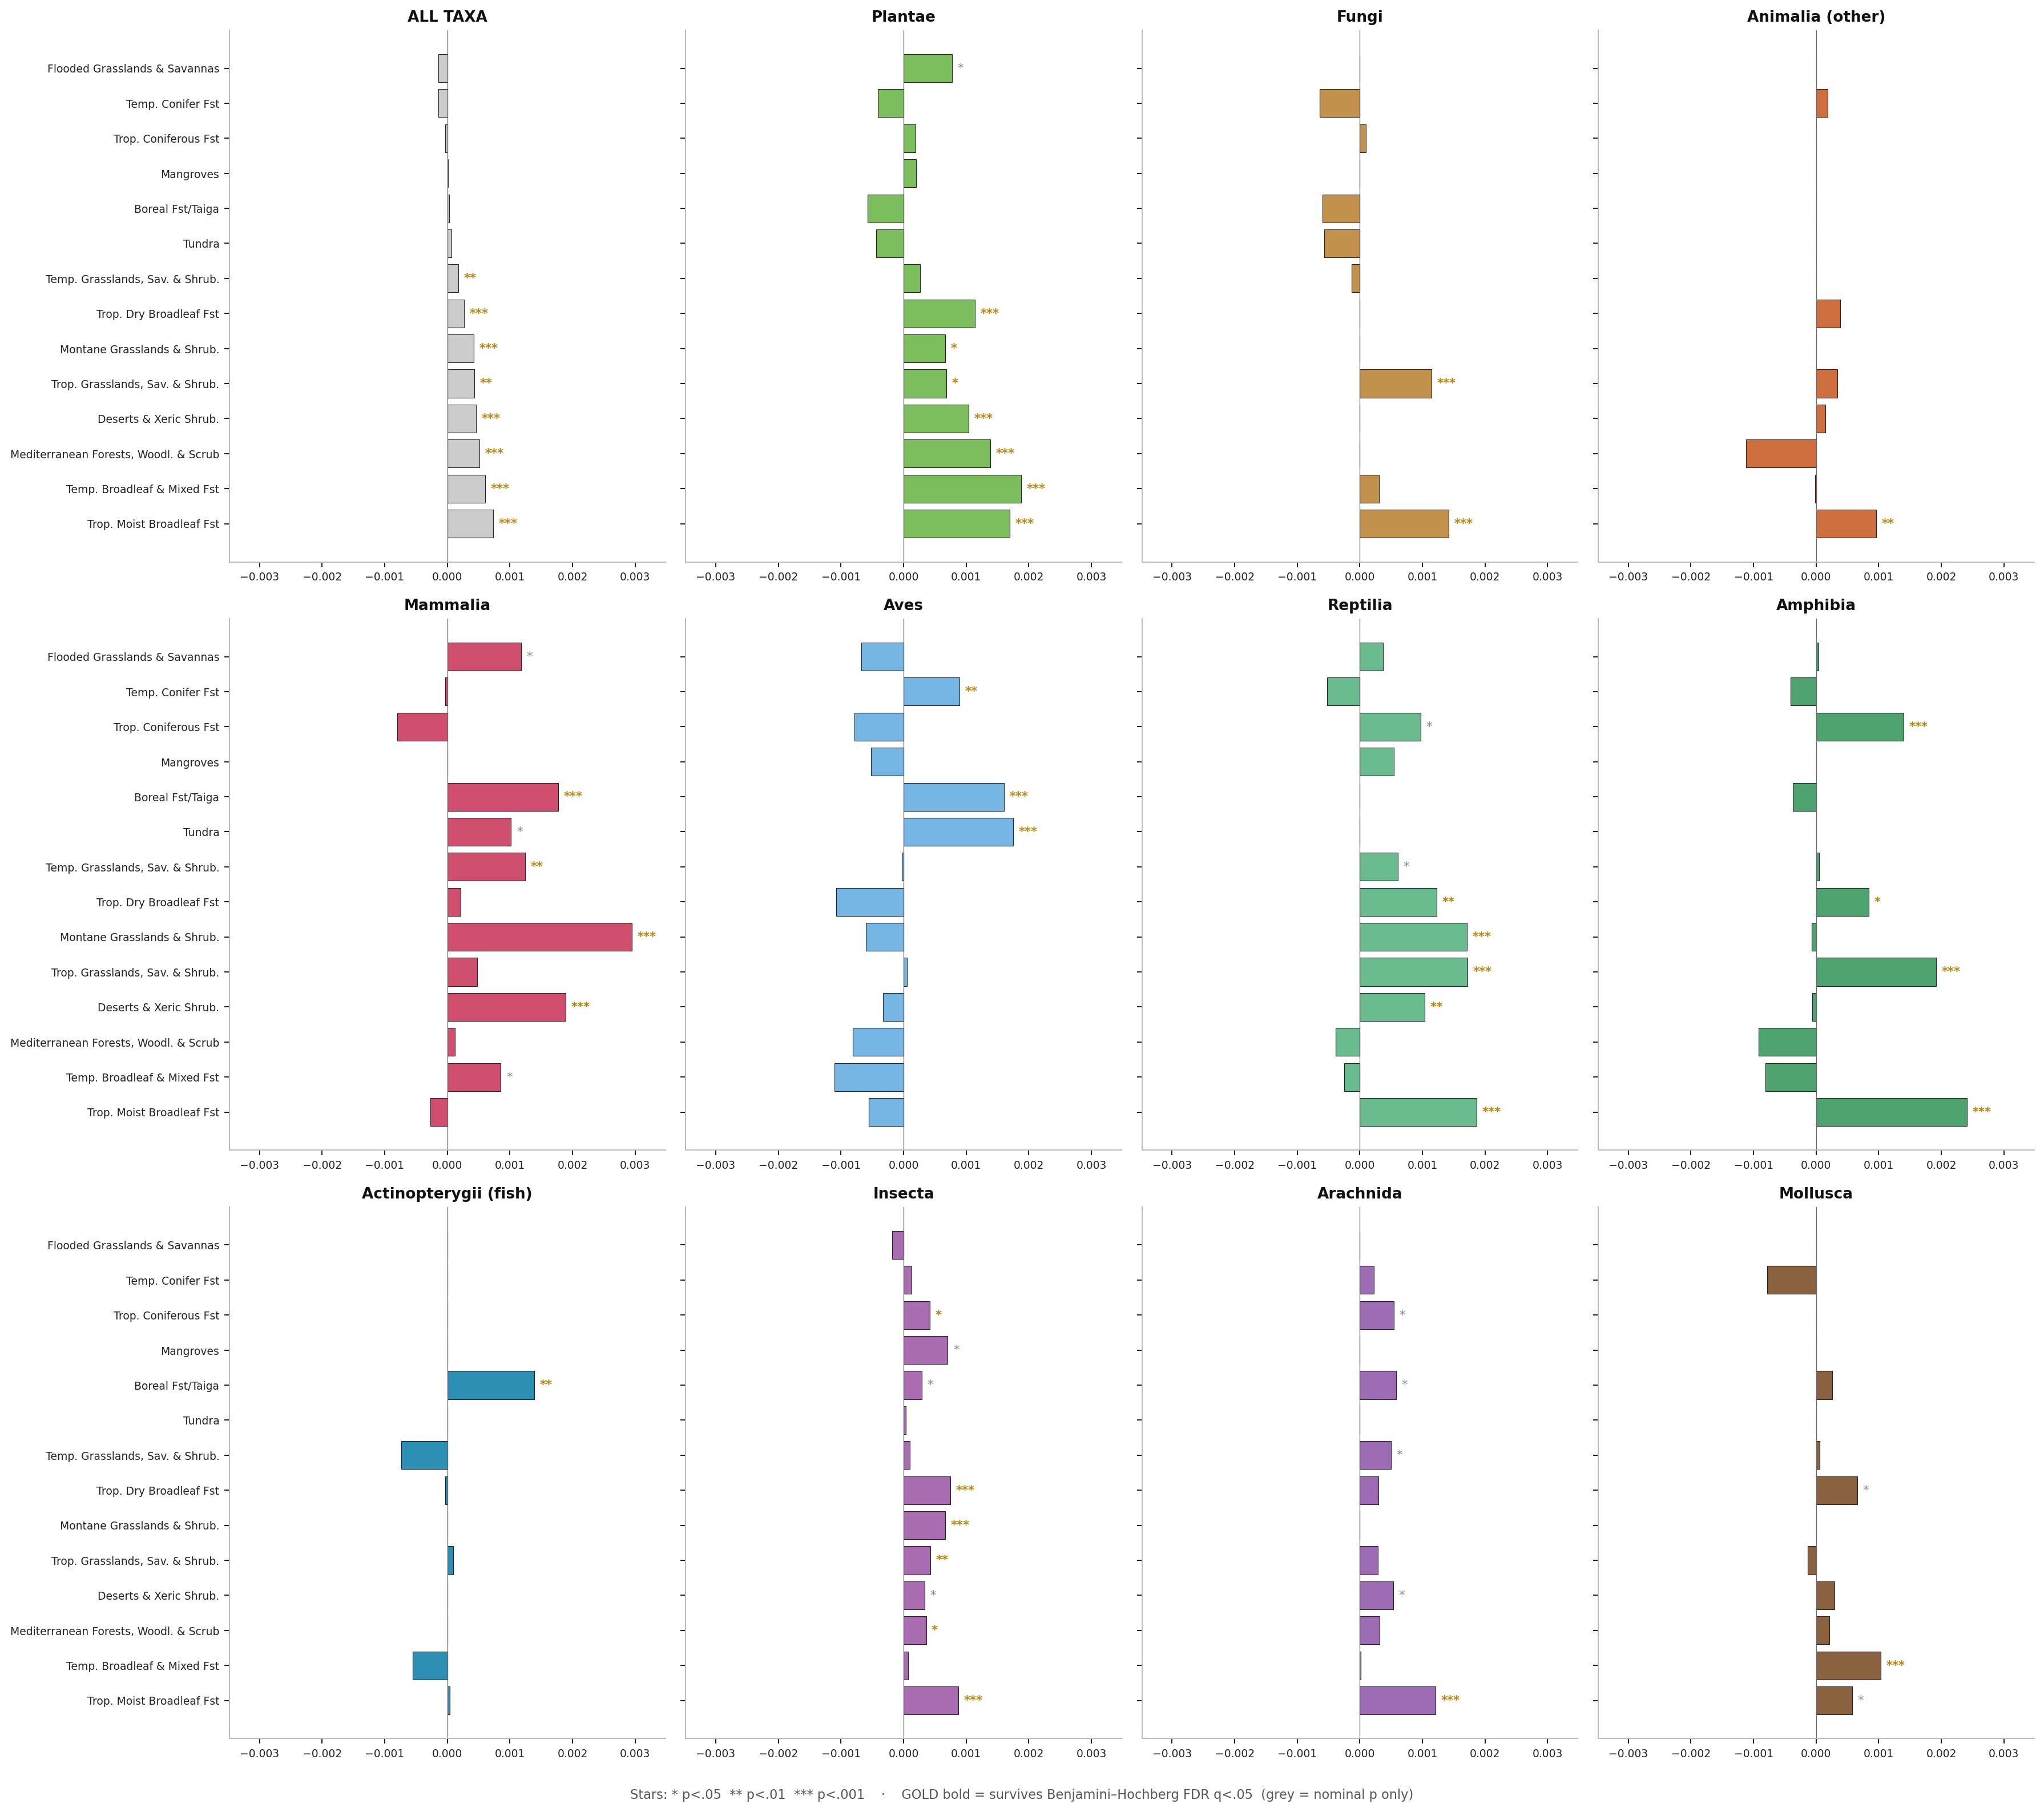
\includegraphics[width=0.95\textwidth]{fig4_taxon_facets.png}
\caption{\textbf{Per-taxon biome panels.} Per-taxon decomposition of
the headline result, presented as small-multiple bar panels with
within-taxon BH-FDR. Each panel shows the per-biome $\Delta$ for one
taxon; biome row order is preserved across panels. Gold stars mark
BH-$q < 0.05$ within the panel. Complements
Figure~\ref{fig:fig10}.}
\label{fig:figS-taxonfacets}
\end{figure}

% S2. Anonymisation-progression robustness ladders removed
% (Fig 8 + Fig 9 in earlier numbering). The naming-progression ladders
% compared the LLM-mediated headline pipeline against earlier
% rule-based hypernym maps (v3 / v4 / v6 / v7 / v8). The progression
% was useful as evidence that the effect is not specific to one
% anonymisation choice, but presenting it alongside the LLM headline
% invites the reader to weigh methods that were subsequently
% superseded. The robustness claim is preserved verbally in the
% Methods section.

\subsection*{S3. Cross-model and cross-language replication}

Figure~\ref{fig:figS-crossmodel} tests whether the across-biome
ranking of $\Delta$ is an artefact of the specific vision-language
model architecture used to produce the embeddings (SigLIP-2-large
in the headline analysis). For this robustness check we re-run
the residualised Spec~A pipeline with four distinct
vision-language model families across two text languages, using
the earlier hand-curated class-level Russian hypernym map (v7)
as the text anonymisation rather than the LLM-mediated pipeline
used in the headline; the per-biome $\Delta$ scale therefore
differs from the headline numbers but the across-biome ranking
is the test of interest. The top row uses the Russian-language
abstracts under SigLIP-2-large and under M-CLIP
(XLM-Roberta-Large paired with CLIP-ViT-L/14). The middle and
bottom rows use machine-translated English one-liner motif
summaries under SigLIP-2-large, OpenCLIP-ViT-L/14 trained on
LAION-2B, and OpenCLIP-ViT-L/14 trained on the OpenAI corpus.
The scatter panels show per-biome $\Delta$ for matched model
pairs. Spearman $\rho$ lies in $[+0.71, +0.82]$ across
cross-model pairs; the biome ranking is preserved across every
model family tested. The across-biome ranking is therefore not
a SigLIP-specific artefact.

\begin{figure}[h!t]
\centering
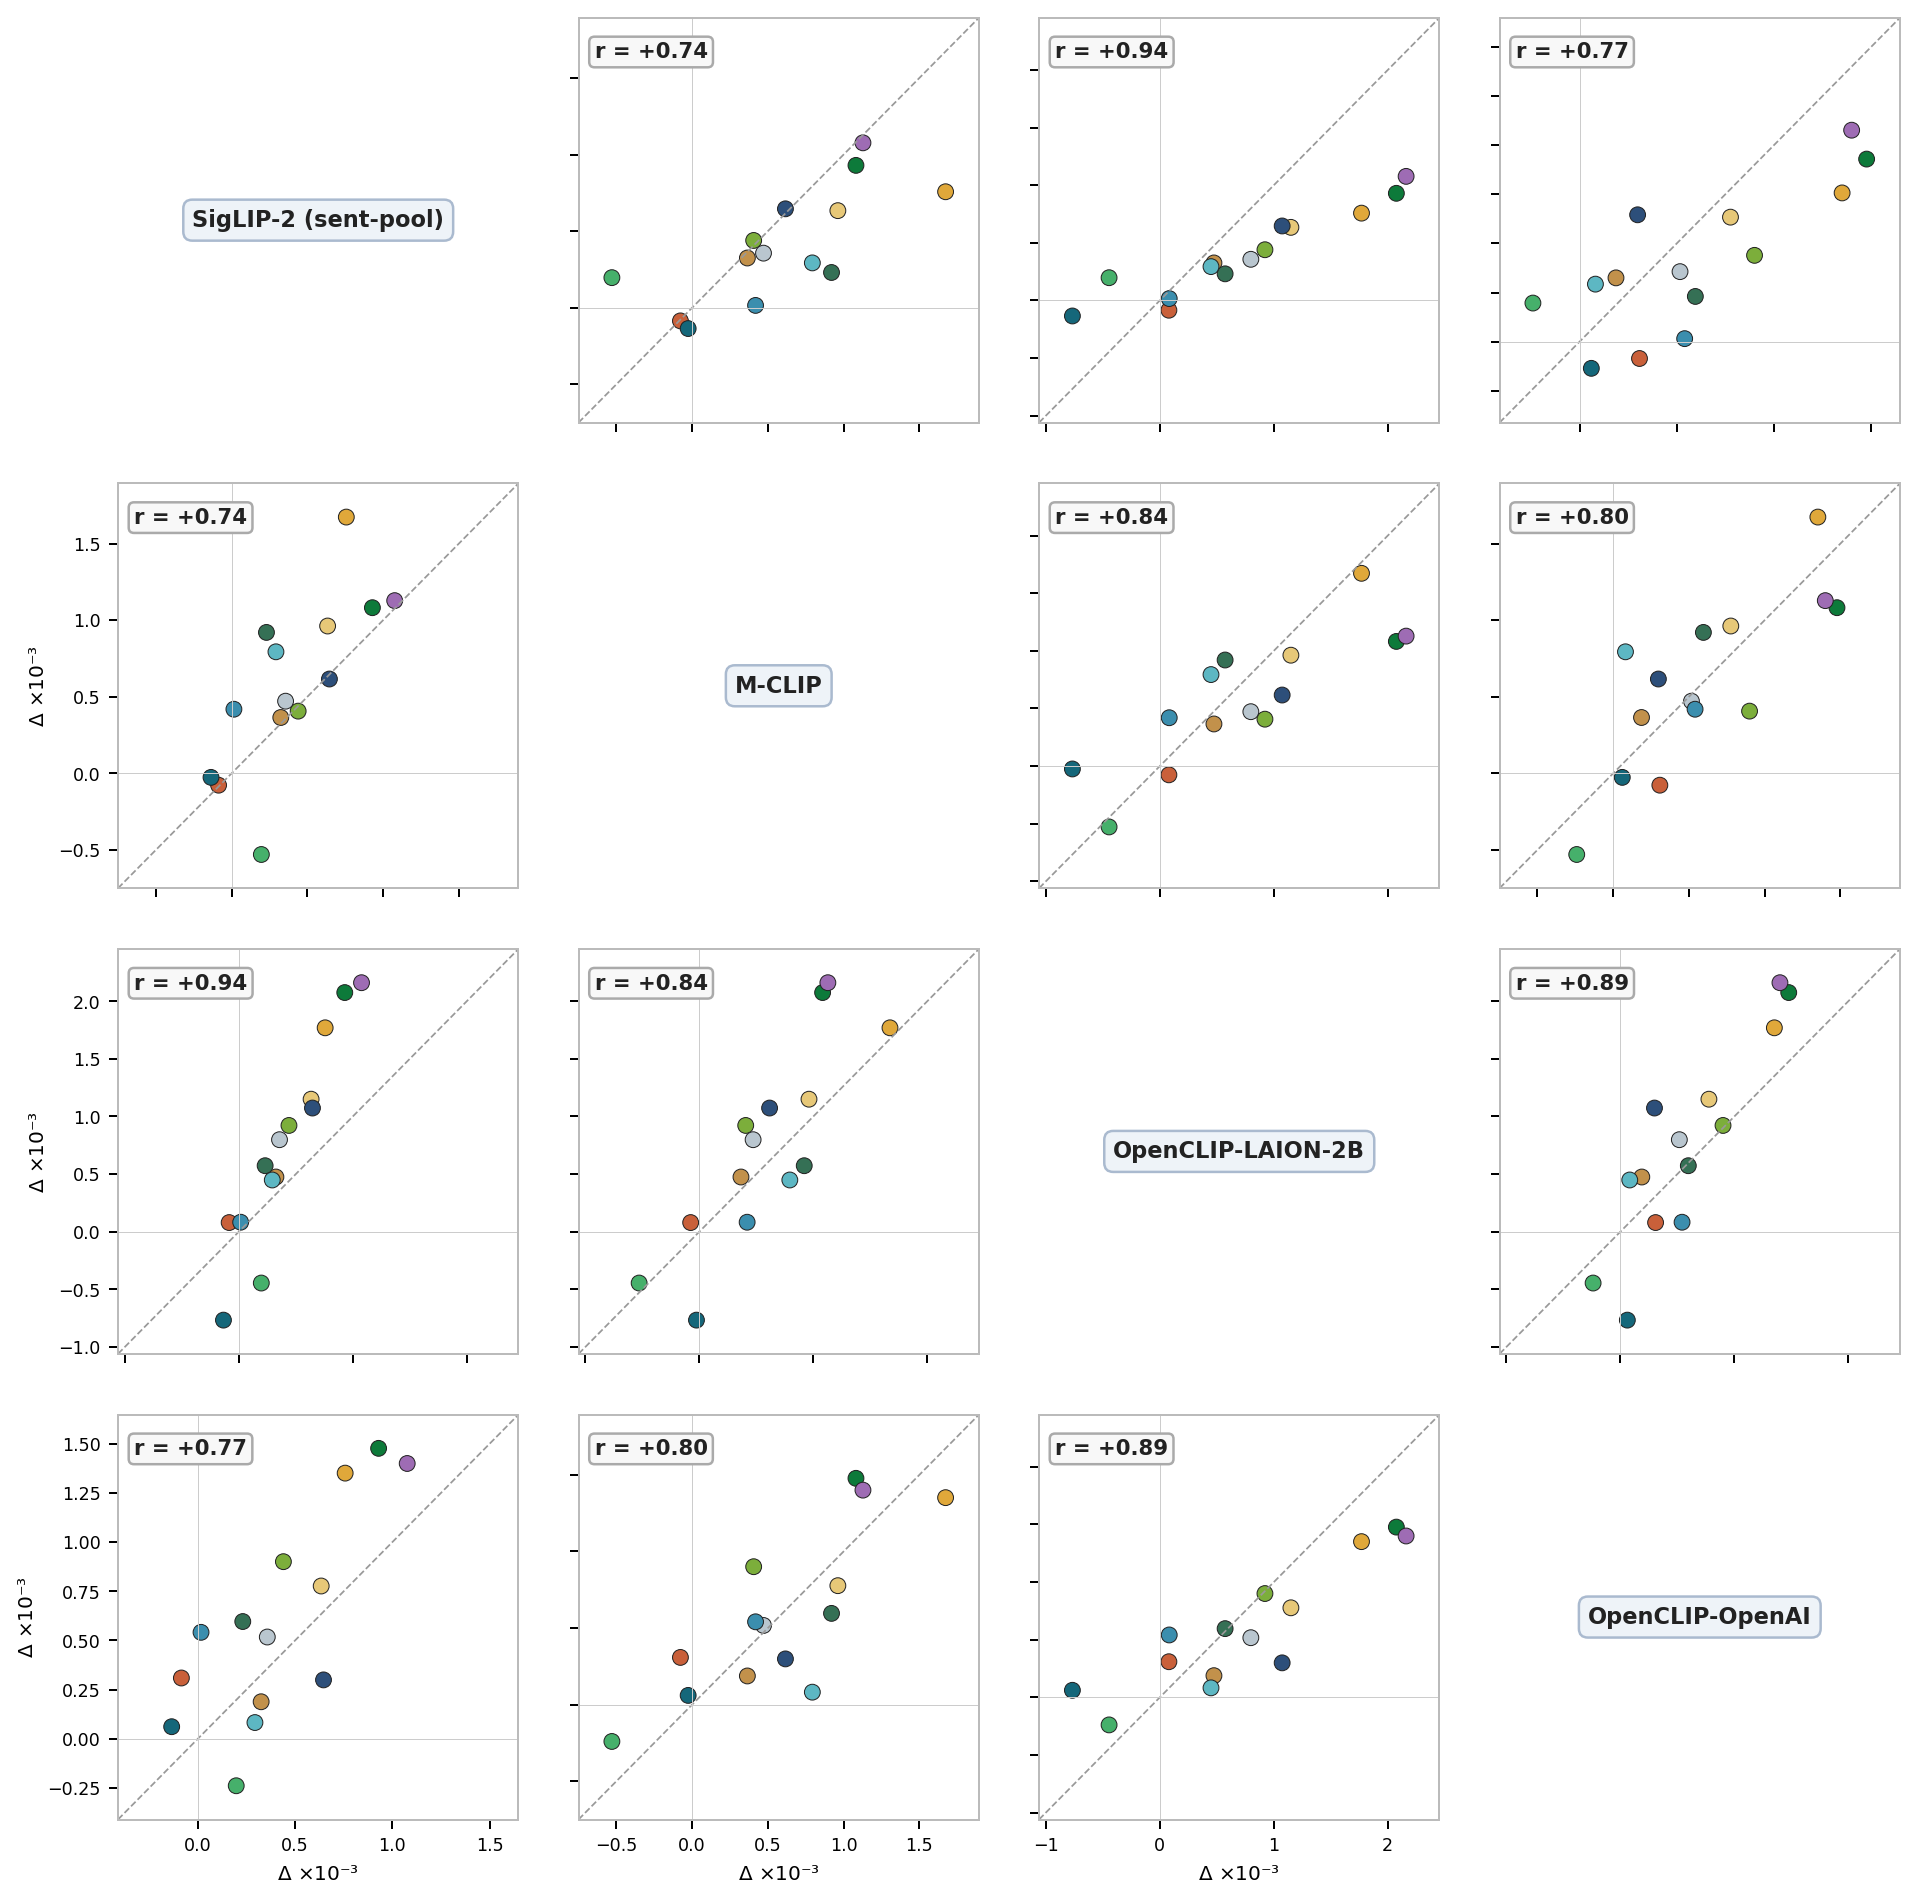
\includegraphics[width=\textwidth]{fig9_crossmodel_correlation.png}
\caption{\textbf{Cross-model robustness.} \emph{Top row}: Russian
abstracts with SigLIP-2-large and M-CLIP (XLM-Roberta-Large +
CLIP-ViT-L/14), plus their per-biome scatter. \emph{Middle row}:
English one-liners with SigLIP-2-large, OpenCLIP-ViT-L/14-LAION-2B,
and OpenCLIP-ViT-L/14-OpenAI. \emph{Bottom row}: per-biome scatters
between SigLIP-2 oneliners and each OpenCLIP model. Spearman $\rho
\in [+0.71, +0.82]$ across all cross-model pairs.}
\label{fig:figS-crossmodel}
\end{figure}

% Whole-corpus residualised panel removed: the headline analysis
% (Figure 2) is now itself computed on the full LLM-clean corpus of
% ~1,921 motifs without any Spec A restriction, so a separate
% supplementary version would be redundant.

\subsection*{S5. Raw ecological composition per biome}

Figure~\ref{fig:figS-species} reports the raw ecological composition
of motif text per biome, before anonymisation. For each WWF biome
(rows) and each of fourteen taxonomic and botanical categories
(columns), the left panel of the heatmap shows the percentage of
Spec~A motifs whose raw Russian abstract mentions at least one
species or plant of that category. The right panel shows the
difference between the Spec~A subset and the all-in-biome pool: a
positive cell means the category is over-represented in
biome-specific motifs relative to the universal-dominated full
pool. The heatmap therefore makes explicit, at the textual level,
which taxonomic categories carry biome-specific signal before the
hypernymisation layer removes their names from the encoder's
input. The figure helps motivate which species-vocabulary
categories the v7 hypernym map needed to cover comprehensively, and
clarifies the ecological content the encoder is no longer
reading at the headline stage.

\begin{figure}[h!t]
\centering
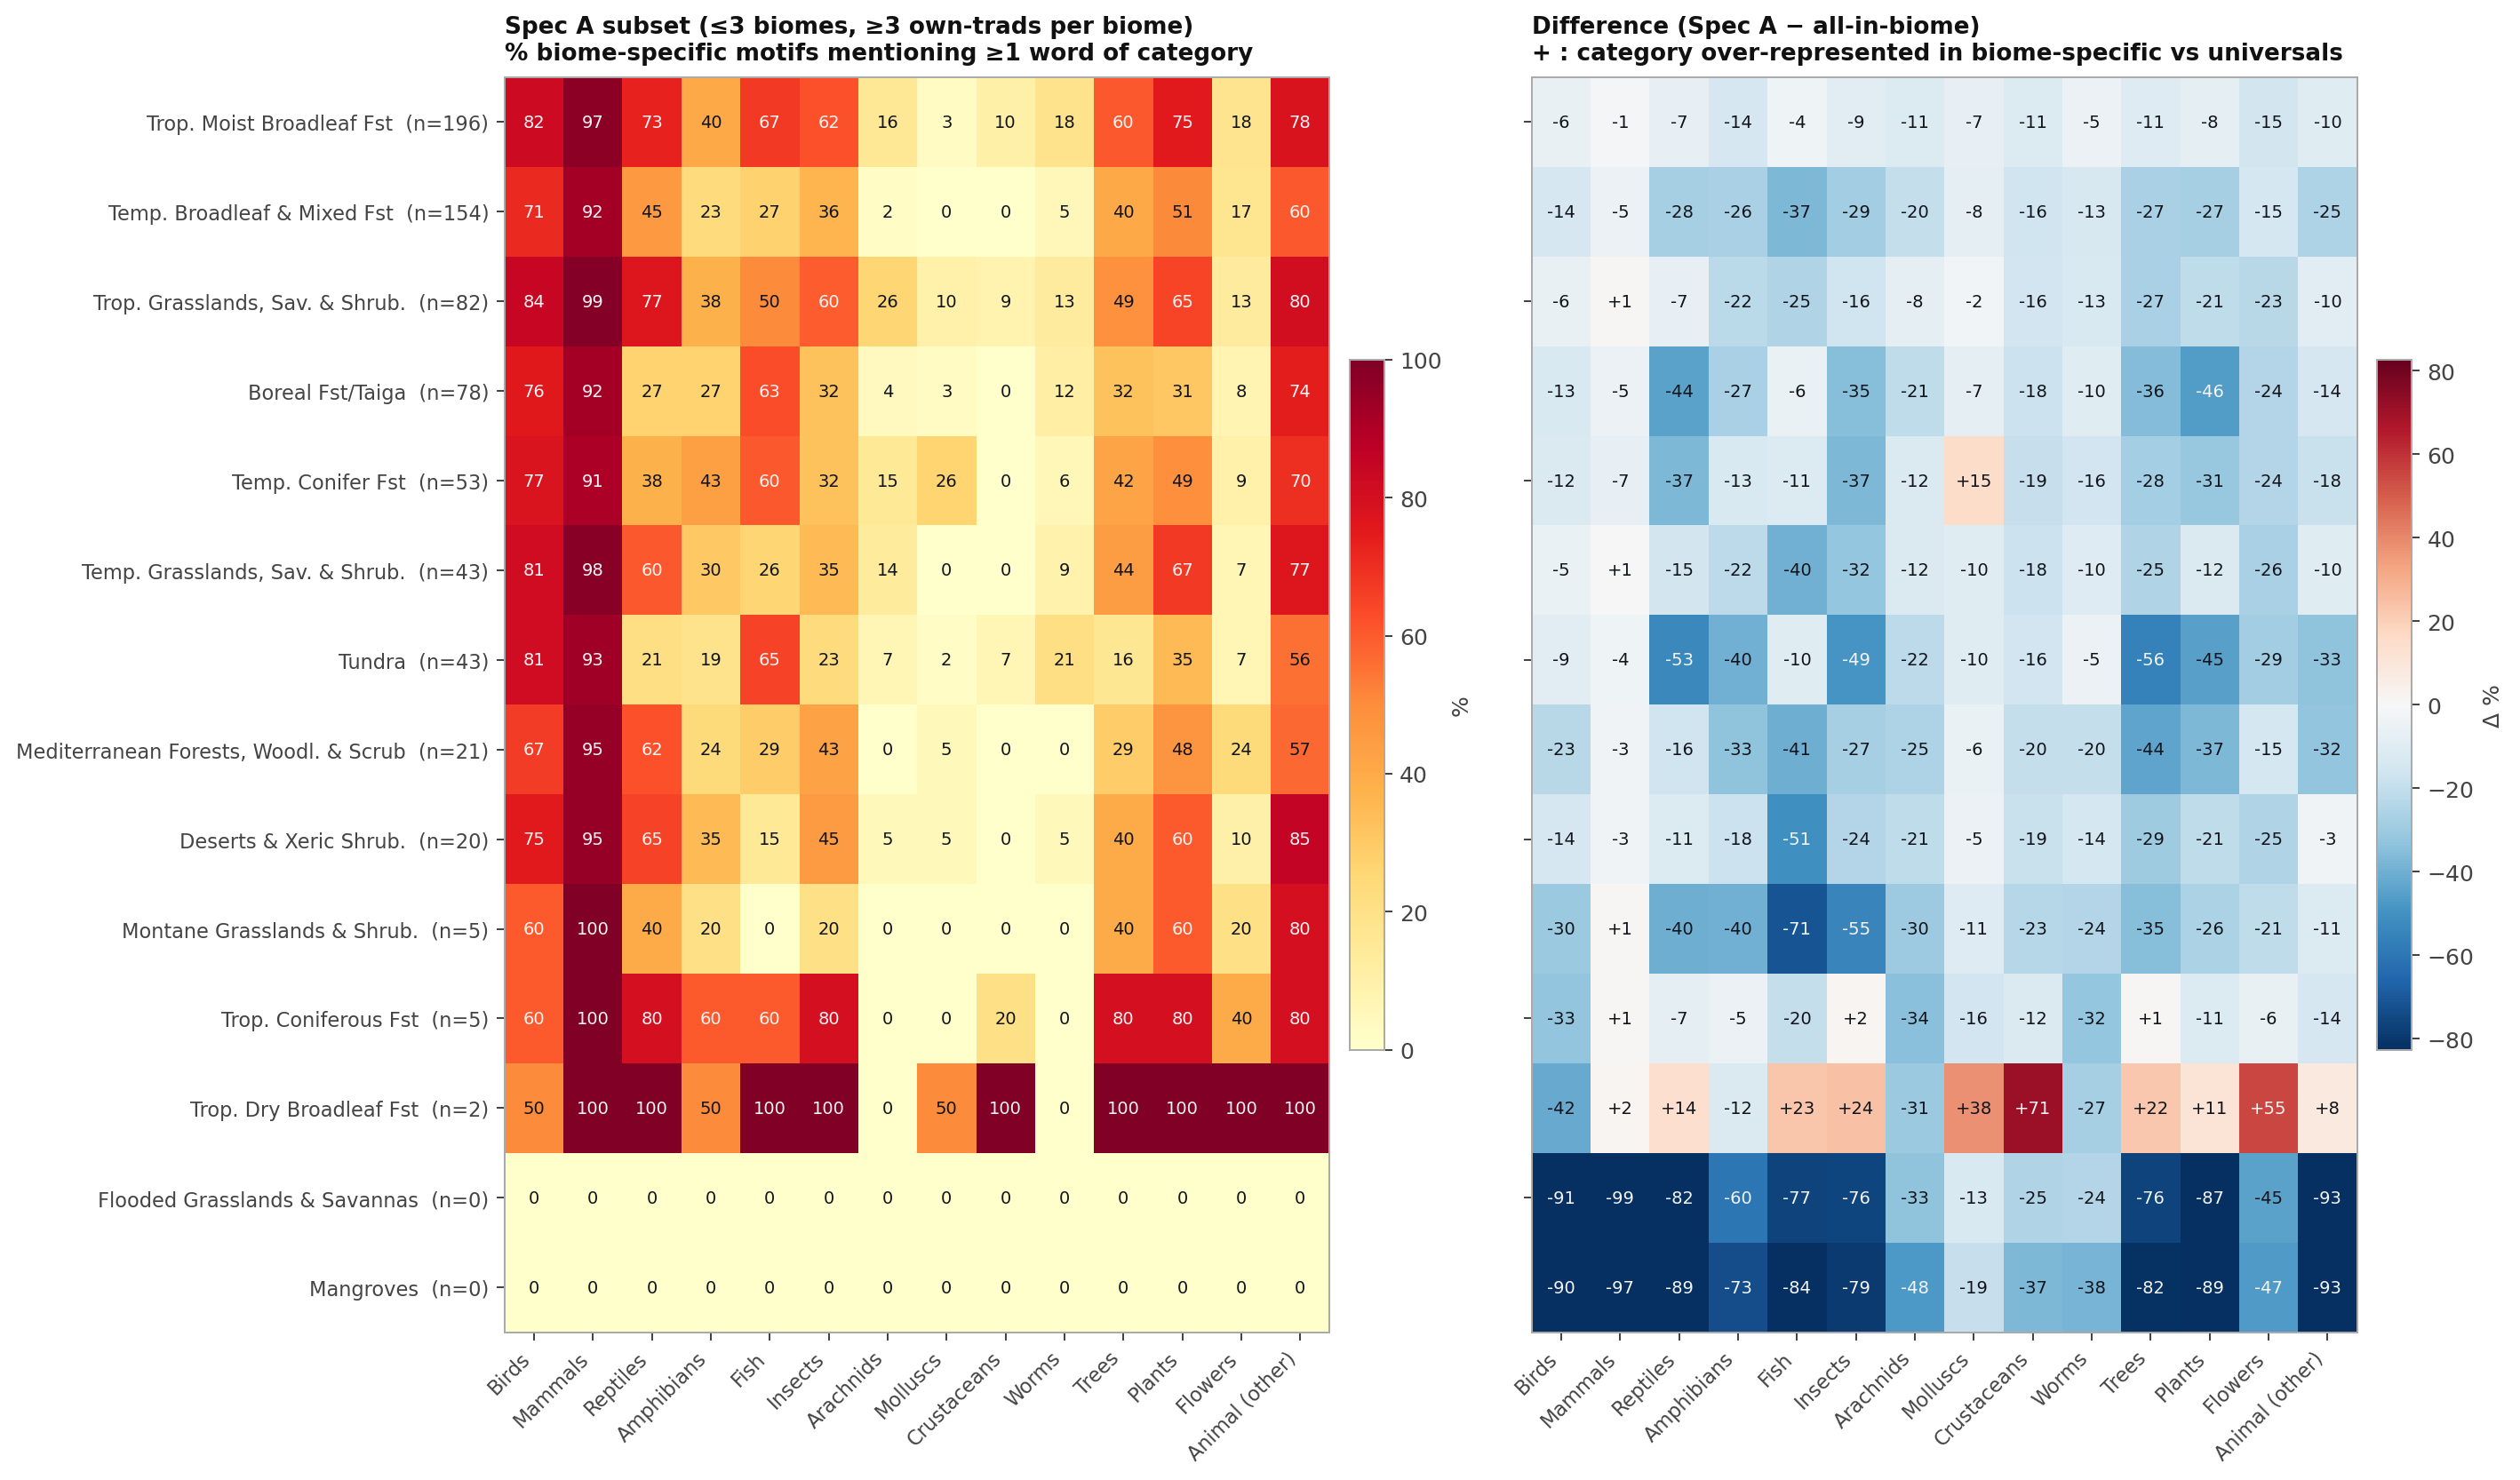
\includegraphics[width=0.95\textwidth]{figS_species_per_biome_specA.png}
\caption{\textbf{Ecological composition per biome (Spec~A subset).}
\emph{Left}: for each WWF biome (rows) and each of 14 taxonomic and
botanical categories (columns), the cell shows the percentage of
\emph{Spec~A motifs} (motifs touching $\leq 3$ biomes, $\geq 3$
own-traditions in that biome, the same selection that drives the
headline result) whose raw Russian abstract mentions at least one
species or plant of that category, before anonymisation.
\emph{Right}: difference (Spec~A minus all-in-biome). Positive cells
mark categories over-represented in biome-specific motifs relative
to the universal-dominated full pool, revealing the ecological
fingerprint that the species-hypernymisation layer subsequently
removes. The all-motifs version of the heatmap is dominated by
universal motifs and therefore uniformly red across biomes; we omit
it here and release the underlying counts in the data drop.}
\label{fig:figS-species}
\end{figure}

\end{document}
